%% ============================================================================
%% main.tex — PSD Framework @ Pattern Recognition 投稿主装配文件
%% 模板: els-cas cas-sc (单栏) — 用户决策 A 定案 2026-08-26（官方 Guide for Authors 直链模板族）
%% 类选项实证: review => setspace + \doublespacing（cas-sc.cls L67/L138），对应 PR
%%   "single-column, double-spaced" 投稿硬约束; 页数窗口 20-35 页含参考文献附录。
%% 引用样式: PR 刊出为数字制 => natbib numbers + elsarticle-num.bst（官方 Elsevier 数字样式）。
%% 装配纪律（2026-09-10 交割）: body truth = 各节 tex 文件（R22 后全部修订直改 tex，md 不回同步）；
%%   docs/paper/<owner>.md 冻结为历史设计稿（头部有治理注记）；全文对账仍以 number-index（gen_number_index.py）为准。
%% 排版纪律: pdflatex 非 Unicode 引擎——排版面（非注释）禁 CJK；占位一律走 \TODO{} 且参数纯 ASCII。
%% 编译: 本目录内执行（latexmk 需 Perl，本机未装——用经典三连）:
%%   pdflatex -interaction=nonstopmode main.tex ; bibtex main ; pdflatex x2
%% ============================================================================

\documentclass[a4paper,fleqn]{cas-sc}
% ^ 2026-11-16 篇幅压缩: 移除 review 选项（review=双倍行距, 59 页超长; final=单倍行距, 30 页达 CVIU 目标）。
%   PR 时代的 "single-column, double-spaced" 约束随改投 CVIU 一并复核; 如需恢复评审版, 加回 review 选项即可。
% 若标题页超一页: 加选项 longmktitle。

\usepackage[authoryear]{natbib}              % 著者-年份引用（CVIU GFA References 节要求 author-year，2026-11-16 复核）
%\usepackage[numbers,sort&compress]{natbib}  % 备选: 数字引用（PR 时代口径）
\usepackage{xcolor}
\usepackage{tabularx}                         % 表格自动换行（tab1/tab2/tab3 版心适配）
\usepackage{algorithm}                        % Algorithm 1 伪代码（03-method）
\usepackage{algpseudocode}

%% 装配占位宏: 红色 TODO 在成稿中必须清零（grep '\TODO{' 即得清单）
\newcommand{\TODO}[1]{\textcolor{red}{\textbf{[TODO: #1]}}}

\graphicspath{{../figures/}}                 % fig1-4 PDF 位于 docs/paper/figures/

%% R31 浮动体修复(交叉重排 2026-09-11): cas-common.sty 的 figure/table 环境依赖
%%   etoolbox \csxdef 回写 \\fps@figure, 裸 [t] 语法走 unknown-key 分支会把定位符写空
%%   (实测 \\fps@figure 运行时 undefined => 全部图表滞留文末浮动页 37-41 的根因)。
%%   双保险: ①\\def 预置合法默认定位符(\\renewcommand 对 undefined 会报错被 nonstopmode 吞掉)
%%   ②全部浮动环境改用类约定的 [pos=t] 键值语法(实测有效)。
\makeatletter
\def\fps@figure{tbp}
\def\fps@table{tbp}
\makeatother

%% 篇幅压缩（2026-11-16）: 浮动体间距微调（标准弹性范围低端）+ 参考文献小字+紧排
\usepackage{setspace}
\renewcommand{\bibfont}{\footnotesize}
\setlength{\bibsep}{2.5pt plus 1pt}
\setlength{\floatsep}{7pt plus 2pt minus 2pt}
\setlength{\textfloatsep}{9pt plus 2pt minus 4pt}
\setlength{\intextsep}{7pt plus 2pt minus 2pt}
\setlength{\abovecaptionskip}{6pt plus 1pt minus 1pt}

\begin{document}

\let\WriteBookmarks\relax
\def\floatpagepagefraction{1}
\def\textpagefraction{.001}

%% ---------------- 前置区（Frontmatter）----------------
\shorttitle{Physics-semantics decoupled framework under evolving evaluation criteria}
%% 排版纪律 2: 前置区字段(shortauthors/author/ead/affiliation)会被类内 LaTeX3 机制全展开——
%%   禁放任何自定义宏(含 \TODO/\textcolor)，只写纯文本占位；\TODO 仅用于正文区。
\shortauthors{Hou et al.}

% R20 标题终裁（模拟审稿最优解）：移除"Low-Resource"——动物层端到端低资源为负，标题词与结果不匹配是 framing 级拒稿面；
%   卖点迁到已交付且新颖的"解耦+演化评估准则"。low-resource 作为设计目标保留在摘要/正文/关键词（上下文即时限定）。
% 2026-11-15 CVIU 改投终裁：标题去掉物种/模态限定（Animal/Skeleton-Based），主张按收缩后口径落在"解耦框架+演化评估准则"。
\title[mode = title]{A Physics--Semantics Decoupled Framework for Behavior Recognition under Evolving Evaluation Criteria}
%% R18: casprelimstitle 在 highlights/abstract prelims 框内不自动折断（类缺陷）——手动断行修复 117pt overfull

\renewcommand{\casprelimstitle}{A Physics--Semantics Decoupled Framework\\ for Behavior Recognition\\ under Evolving Evaluation Criteria}%% R18 fix: 类不重排此框内标题, 手动三段断行全部落在 \textwidth 内, 消除 117pt overfull

%% 作者区 USER 终审项: 名单/单位/ORCID/通讯标记——结构按官方模板预留
\author[1]{Zhimai Hou}[orcid=0009-0006-1360-8359]
\cormark[1]
\ead{3389812293@qq.com}
\credit{Conceptualization, Methodology, Software, Validation, Formal analysis, Investigation, Data curation, Visualization, Writing -- original draft}
\affiliation[1]{organization={Yunnan Police College},
            city={Kunming},
            postcode={650000},
            country={China}}
\cortext[1]{Corresponding author}
\cortext[2]{Corresponding author}
\author[2]{Jinhuan Wu}
\credit{Writing -- review \& editing}
\affiliation[2]{organization={Qujing Normal University},
            city={Qujing},
            postcode={655000},
            country={China}}
\author[3]{Ying Geng}
\cormark[2]
\ead{gingying@sjtu.edu.cn}
\credit{Writing -- review \& editing}
\affiliation[3]{organization={Shanghai Jiao Tong University},
            city={Shanghai},
            postcode={200240},
            country={China}}
\author[4]{Guoliang Yang}
\credit{Writing -- review \& editing}
\affiliation[4]{organization={Beijing University of Chemical Technology},
            city={Beijing},
            postcode={100029},
            country={China}}
\author[5]{Shuo Lin}
\credit{Writing -- review \& editing}
\affiliation[5]{organization={Southwest Jiaotong University},
            city={Chengdu},
            postcode={610031},
            country={China}}
\author[6]{Jiabin Zhao}
\credit{Writing -- review \& editing}
\affiliation[6]{organization={Criminal Investigation Police University of China},
            city={Shenyang},
            postcode={110035},
            country={China}}
\author[7]{Ting Yang}
\credit{Writing -- review \& editing}
\affiliation[7]{organization={Southwest University},
            city={Chongqing},
            postcode={400715},
            country={China}}
\author[1]{Chengze Lyu}
\credit{Writing -- review \& editing}
\affiliation[1]{organization={Yunnan Police College},
            city={Kunming},
            postcode={650000},
            country={China}}

%% ---------------- 摘要（2026-11-16 统稿: 词数见下注; 归因叙事与 tab:attribution-controls 对齐——TRANS-002 同 episode 读数
%%   75.3/79.8/82.6 与同 episode 零重训 remap 界 68.0%（E1 实测, runs/p1_sprint/zerobound_6049）如实写入;
%%   60→10 coarse-grouping 的 76.8% 与 60→49 不同 episode, 摘要不再使用;
%%   剩余价值主张按 E3 + k 阶梯 E3b 实测定稿（runs/p1_sprint/split_addition_episode, runs/p1_sprint/k_ladder）:
%%   全梯度无平价 → 摘要如实写 "residual-value hypothesis not supported at any budget", decoupled 仅余成本节省;
%%   已删: 设问句 "This paper asks..."、线性头归因括注（nuance 保留于贡献3/结论/E9 正文）、"an honest negative result" 尾注。
%%   词数（空白分词、数学组记 1、em/en-dash 不拆）=242，保守口径（em/en-dash 拆开）=247，两口径均 ≤247（余量 ≥3）
%%   （2026-11-16 P1 终审删词复测：删 "measured"/"tested" 各 1 词、"never within"→"outside"（−2）、
%%   删 "at a large accuracy cost"（同句 45.3–72.4 vs 95.9 已量化该成本）；计数法：剥 \textbf/\emph 壳保内容、
%%   其余命令与 $ 脱壳、空白分词、含字母数字判词（脚本 scripts/p1_sprint/count_abstract_words.py）；
%%   投稿系统计数可能有 ±2 出入）----------------
%% 2026-11-16 P1 头对头更新: NTU60 句嵌入外部基线对比（re-implemented AimCLR 66.7 / supervised ST-GCN 66.5, PSD 67.5;
%%   full-budget 监督 83.5 占优如实写入）, 并为控词数微调压缩（merge 句改 equal-budget alternatives、controls 句紧凑化）。
\begin{abstract}
Evaluation criteria in behavior recognition keep evolving; taxonomy changes re-open annotation and retraining. We propose PSD, a physics--semantics decoupled framework for skeleton-based behavior recognition: a label-free physics layer learns \emph{how skeletons move}; a semantic layer learns \emph{what behaviors are called} from rule-engine seeds via clustering, confidence-filtered pseudo-labels, and warm-started self-training. A pre-registered, tier-separated protocol reports cost against accuracy and publishes failures. A synthetic-tier taxonomy transition is absorbed at \textbf{$\geq$3$\times$ lower retraining cost than full retraining} ($6.07\times$). Controls attribute the savings to semantic rebuilding, not freezing (naive freezing: 68.6\% vs.\ 98.2\%). On the real merge transition the decoupled rebuild (75.3\%) trails equal-budget alternatives (coupled 79.8\%, matched-solver 82.6\%); the same-episode zero-retraining bound reads 68.0\% (10\% head budget). On split/addition transitions, a labeled-budget ladder (10--100 labels/class) lifts the decoupled rebuild from 45.3\% to 72.4\% versus coupled 95.9\%---outside the $\pm$2.3\,pp parity band: the residual-value hypothesis is \emph{not supported at any budget}, and decoupling buys only label and wall-clock savings. The warm-started semantic layer reaches \textbf{82.0\% top-1 on 22 classes from 20 clips} (vs.\ \textbf{96.6\% full-budget}). A frozen-feature pipeline retains \textbf{90.7\% of full-budget linear-probe accuracy at 10\% labels} on NTU60 (88.9\% NTU120; 85.8\% PanAf500)---above re-implemented AimCLR (67.5\% vs.\ 66.7\%) and supervised ST-GCN (66.5\%), though full-budget supervision dominates (83.5\%)---collapses on UCF101 (66.6\%), and stays \emph{below chance} on the canine tier at 13\% budget (9.8\% vs.\ 11.1\% chance). Decoupling pays where a frozen backbone is reusable and semantics rebuild cheaply; the protocol exposes where it fails.

\end{abstract}
%% [E1-INTERFACE·已消费 2026-11-16 统稿] E1（TRANS-002 同 episode 60→49 零重训界重测）已出数并回填三处：
%%   rename-oracle 上界 68.04% / argmax-vote 下界 67.97%（10% 标注头预算, seed 42, 纯推理 112.5s, 零重训零新标注）。
%%   数值源 runs/p1_sprint/zerobound_6049/summary.json（reports/p1_sprint_evidence/ 有逐字节一致副本）, 严禁编造。
%%   同步点: 本摘要句 + 01-introduction.tex 贡献1 + 06-conclusion-limitations.tex 结论段与 L12 + 04-experiments.tex
%%   tab:attribution-controls（60→49 界两行）。60→10 的 76.8%/76.5% 仍是另一 episode 的合法数字, 不可混用。
%% [E3b-INTERFACE·已消费 2026-11-16 统稿] k 阶梯（E3b: 同 split/addition episode 定义, k∈{10,25,50,100} 新标注/类,
%%   池扩到 100/类支持 k=100, k=10 档为趋势参照非 E3 复现）: decoupled 45.3/59.1/65.1/72.4%（全部档位三种子 42/43/44, std ddof=0; k=100 ±0.0）,
%%   coupled 95.9%（±0.5, k 无关参照）, frozen-head 71.7%；coupled−decoupled 边际 50.57/36.78/30.80/23.45pp,
%%   全梯度落在 ±2.3pp 平价带外 → k*=None（verdict=no_parity_within_tested_range）。
%%   摘要剩余价值句据此降级为 "not supported at any tested budget"；decoupled 仅余标注/墙钟节省
%%   （k=10: 100 vs 1000 新标注, 92s vs 234s, seed 42）。
%%   数值源: runs/p1_sprint/k_ladder/summary.json（reports/p1_sprint_evidence/ 有副本）, 严禁编造。
%%   同步点: 本摘要句 + 01-introduction.tex 贡献1 + 04-experiments.tex（Reinforcement E3/E3b 段 + tab:kladder）
%%   + 06-conclusion-limitations.tex 结论段与 L12 + supplementary.tex app:kladder。
%% [FROZEN-REAL·已消费 2026-11-16] 摘要冻结句（NTU60 90.7%; NTU120 88.9%; PanAf500 85.8%; UCF101 66.6%）由本轮真实 tier
%%   frozen-encoder 对照执行支撑: runs/p1_sprint/{ntu120,ucf101,panaf500}/summary.json（三臂 C/A/B, trainable=0 断言,
%%   与 2026-09-07 已报告 E9 值逐位一致）; 协议全文 supplementary app:frozenreal。摘要正文未改（数字本已多 tier 一致）。

%% Highlights 同步维护两处: 此处（版内）+ highlights.tex（投稿系统独立可编辑文件）
%% 2026-11-15 深度改造: R2-1/R2-5 联动——6.07x 显式限定 synthetic tier；82.0% 补 full-budget 对照；k-NN 降位并标 probe。
\begin{highlights}
\item Decoupled framework absorbs taxonomy evolution cheaply (synthetic tier)
\item Taxonomy transitions cost $\geq$3x less wall clock (measured 6.07x, synthetic tier)
\item Warm start: 82.0\% top-1 from 20 clips (vs.\ 96.6\% full-budget, offset tier)
\item NTU60 frozen features retain 90.7\% at 10\% labels, above AimCLR and ST-GCN baselines
\item Canine tier stays below chance at 13\% budget (9.8\% vs.\ 11.1\%)---honest boundary
\end{highlights}

%% 关键词（2026-11-16 回修重排: 与收缩后的主张对齐——去掉 animal-behavior 领衔与 low-resource 承诺，1-7 个允许）
\begin{keywords}
decoupled architecture \sep skeleton-based action recognition \sep taxonomy evolution \sep pseudo-labeling \sep self-supervised learning \sep evaluation protocol
\end{keywords}

%% 2026-11-15 117pt overfull 根因修复: 该 warning 并非标题断行, 而是 els-cas review 版式把 ARTICLE INFO/keywords 盒
%%   放进 \hbox to 0pt（设计上悬挂于摘要左栏; 盒宽恰为 0.25\textwidth=117.0831pt; 诊断: 去掉 keywords 环境重编译,
%%   该 warning 消失, 其余 overfull 为 0）。属类机制性假阳性: 在 \maketitle 期间临时放宽 \hfuzz 精准豁免该盒,
%%   之后立即恢复默认严格度, PDF 输出不变。
\hfuzz=120pt
\maketitle
\hfuzz=0.1pt

%% 篇幅压缩: 正文行距 0.94（单倍行距范畴内微调; \begin{document} 后设置以确保生效）
\setstretch{0.94}

%% ---------------- 正文装配区（truth = 各节 tex，2026-09-10 交割）----------------
% 01-introduction.tex — truth: 本文件（2026-11-15 深度改造：主张收缩为 taxonomy 演化下物理-语义解耦的成本-收益边界与透明评估协议；犬类负结果前置为边界条件；贡献列表同步收缩）
% 纪律: Para1-6 六段式逐块搬运; Hero figure fig1 落 §1 尾（figure-specs.md 规格）; 数字禁改写。
% Abstract 已在 main.tex 前置区，本节从 Introduction 正文开始。label 沿用桩定义 sec:intro。
\section{Introduction}\label{sec:intro}

Deployed behavior-recognition pipelines rarely face a fixed definition of what they recognize. Working-dog programs redefine behavior categories as training standards evolve; welfare protocols split or merge classes as regulations change; veterinary research adopts finer ethograms as instruments improve. Each such revision re-opens the annotation and retraining pipeline behind the classifier. The economics are unforgiving: training a working dog costs tens of thousands of dollars per animal, and more than half of candidates fail to graduate~\citep{grimm2026science}, so the measurement layer around these programs is both expensive and subject to recurring re-specification.

This paper studies a structural response to that recurring cost: factorize the pipeline so that the part that must track the taxonomy is small. We examine the physics--semantics decoupling pattern, PSD, for skeleton-based behavior recognition under evolving evaluation criteria. A physics layer $\Phi$ learns \emph{how skeletons move} without behavior labels: self-supervised pretraining adapted to quadruped topology plus unsupervised motion-word segmentation that cuts streams into behavior proposals. A semantic layer $\Omega$ learns \emph{what behaviors are called} from a small seed budget: rule-engine coarse labels seed class anchors, prototype clustering assigns pseudo-labels under confidence filtering, and iterated expansion operates within an annotation budget of 100--200 clips; a warm-start protocol initializes this stage from prior semantic-layer weights, making budgets as small as 20 clips usable on the synthetic-offset tier (the canine-tier outcome at a comparable budget is reported in Section~\ref{sec:experiments}). Because the layers interact only through embeddings and proposals, a taxonomy transition $\mathcal{Y}\to\mathcal{Y}'$ retrains $\Omega$ while $\Phi$ remains frozen.

The question this paper answers is deliberately narrower than ``does decoupling work?''. Any design that freezes a backbone and retrains a head inherits the same computational shortcut at a taxonomy change, so the wall-clock ratio alone does not justify the mechanism; and a pre-registered real-domain replication shows the shortcut can invert at small scale, where there is no retraining cost left to save (Section~\ref{sec:experiments}, E6-real). We therefore treat decoupling as a cost--benefit hypothesis with explicit boundary conditions: it pays where a frozen physics layer remains reusable and semantics are cheap to rebuild, and it fails where pseudo-label quality collapses. The contribution is a measured boundary (where the cost advantage holds, where accuracy holds, and where the pipeline breaks), established under a pre-registered, tier-separated protocol whose decision rules, tolerances, and negative results are reported in full.

\paragraph{Why animal skeletons, and where the boundary lies.}
Animal behavior recognition motivates the problem: labeled behavior data is scarce, skeletons are the practical signal, and evaluation criteria in working-dog and welfare settings evolve with operational practice (Section~\ref{ssec:rw-animal}). On the only public canine behavior tier we could assemble, the end-to-end pipeline stays below chance at a 13\% annotation budget (\textbf{9.8\% $\pm$ 7.5 against an 11.1\% chance level}, with a generic-SSL control reaching \textbf{15.2\% $\pm$ 5.1}), and a pre-registered diagnosis attributes the failure to label misalignment in the sole public source of canine behavior video with action labels, not to skeleton quality (Section~\ref{sec:experiments}, E7; Section~\ref{sec:conclusion}, L9). We report this as a boundary condition, have pre-registered the target-domain working-dog pilot for a later study, and scope every positive claim to the tiers where it was actually measured rather than claiming a general solution to animal behavior recognition.

Our contributions are threefold:
\begin{enumerate}
\item \textbf{A cost--benefit boundary for physics--semantics decoupling under taxonomy evolution.} On the synthetic tier, a taxonomy transition is absorbed at $\geq 3\times$ lower wall-clock retraining cost than full-pipeline retraining at matched accuracy (conservative bound backed by a measured $6.07\times$; same-seed paired ratios never below $3.99\times$). This bound is a synthetic-tier measurement: real-domain replications return FAIL at MLP scale (no cost to save) and PARTIAL at backbone scale (cost line cleared, accuracy band not exactly matched), so the claim is scoped, not universal.

A pre-registered merge/rename analysis sharpens the boundary. For transitions expressible as label remaps or logit aggregation, zero-retraining upper bounds apply. On the one real merge transition we measure, a matched-solver control bounds the decoupled rebuild from above (82.6\% vs.\ 75.3\%), and the zero-retraining remap bound measured on the same episode reads 68.0\%, below the rebuild; the rebuild is therefore not dominated by the zero-cost path on this episode.

A synthetic split/addition episode probes the residual value of decoupling where new supervision is unavoidable: the zero-retraining remap cannot name the new classes (0\%), and the decoupled rebuild recovers 45.7\% overall with 10 new labels per class, at $3.0\times$ lower median wall-clock and $5\times$ fewer new labels than full retraining (97.1\%; a frozen head with the full new-label budget: 68.0\%). A labeled-budget ladder on the same transition type ($k\in\{10,25,50,100\}$ fresh labels per new class) raises the decoupled arm from 45.3\% to 72.4\% (three seeds 42--44 per rung) but saturates at the frozen-feature ceiling (frozen-head arm: 71.7\%) and never approaches the coupled arm (95.9\%). The smallest margin, 23.45\,pp at $k{=}100$, sits far outside the $\pm2.3$\,pp parity band, so the residual-value hypothesis fails across the entire tested ladder; decoupling's measured value in this regime is label and wall-clock savings, and closing the gap appears to require adapting the frozen encoder (seeds 42--44; Section~\ref{sec:experiments}).

The cost of freezing itself is likewise measured. A frozen-encoder control on the three real E9-series tiers (NTU120, UCF101, PanAf500) shows naive freezing retains only \textbf{88.9\%/66.6\%/85.8\%} of full-budget accuracy under the interim supervised encoder, and a protocol-return amendment executing the pre-registered label-free physics layer on NTU120, UCF101, and PanAf500 reads \textbf{75.0\%/51.1\%/82.5\%} (all \textbf{FAILS}; Section~\ref{ssec:boundary}).
%% [E3-INTERFACE·已消费 2026-11-16] 贡献1 的假设从句已按 E3 实测替换为实证句：
%%   remap 新类 0% / decoupled(k=10) 45.7% @100 新标注（三种子 0.4448/0.4345/0.4931 均值 0.45747，两位小数 45.75%）/ frozen head 68.0% / coupled 97.1%；
%%   墙钟中位 50.6s vs 153.0s = 3.0×；新标注 100 vs 500 = 5×。seeds 42/43/44。
%% 数值源: runs/p1_sprint/split_addition_episode/summary.json（reports/p1_sprint_evidence/ 有逐字节一致副本）。
%% [E3b-INTERFACE·已消费 2026-11-16] 贡献1 剩余价值句按 k 阶梯（E3b）实测降级：
%%   decoupled 45.3/59.1/65.1/72.4%（k=10/25/50/100；全部档位三种子 42/43/44，std ddof=0；k=100 ±0.0），coupled 95.9%（±0.5，k 无关参照），
%%   frozen-head 71.7%；最小边际 23.45pp@k=100，全梯度落在 ±2.3pp 平价带外 → k*=None，
%%   verdict=no_parity_within_tested_range → "residual-value hypothesis not supported at any tested budget"。
%% 数值源: runs/p1_sprint/k_ladder/summary.json（reports/p1_sprint_evidence/ 有副本），严禁编造。
%% 三处联动已同步（2026-11-16 统稿）: main.tex 摘要句（同 episode 界 68.0%@10% 标注头预算 + E3/E3b 降级式剩余价值）与
%% 06-conclusion-limitations.tex（结论段 + L12）均已改为同口径；60→10 的 76.8% 仅保留为另一 episode 的合法数字。
%% [FROZEN-REAL·已消费 2026-11-16] 贡献1 尾句新增冻结代价实测: 三真实 tier frozen-encoder 对照 88.9/66.6/85.8%（PARTIAL/FAILS/PARTIAL）。
%% 数值源: runs/p1_sprint/{ntu120,ucf101,panaf500}/summary.json（与 2026-09-07 已报告 E9 值逐位一致）;
%% 正文载体: ssec:boundary 冻结对照 bullet + tab:attribution-controls 真实 tier 块; 协议全文 supplementary app:frozenreal。
\item \textbf{A transparent, pre-registered evaluation protocol for tier-separated claims.} Three tiers (synthetic, public-real, real-K9) plus public benchmarks are never pooled; every comparison carries its caliber (label space, budget definition, device, seed dispersion); cost is reported as a pair (annotation units, wall-clock) at matched accuracy; and decision rules (including the conservative $\geq 3\times$ bound, the FULL/PARTIAL/FAIL verdicts, and Holm-corrected families) are frozen before runs. Negative results are first-class findings: the canine-tier collapse below chance, the null rescue levers, and the retention collapse on weak-reference domains (UCF101 66.6\% interim encoder; 51.1\% label-free) are reported under the same rules that certify the positive results.
\item \textbf{An honest empirical map of where the mechanism pays.} Positive evidence: the warm-started semantic layer reaches 82.0\% top-1 on 22 classes from 20 labeled clips on the synthetic-offset tier (vs.\ 96.6\% full-budget; a marginal budget atop a fully labeled source domain), and the end-to-end pipeline retains 90.7\% of full-budget linear-probe accuracy at 10\% of the labels on the human benchmark (75.0\% on NTU120 under the pre-registered label-free physics layer, vs.\ 88.9\% under a disclosed interim supervised encoder; 85.8\% on PanAf500 at thirty seeds (interim encoder; 82.5\% under the pre-registered label-free physics layer), ten-seed readout released alongside); separately, a linear head on frozen features alone retains 88.7\% on NTU60. Under the identical budget protocol the 10\% semantic arm also edges re-implemented published-method baselines, AimCLR linear evaluation (67.5\% vs.\ 66.7\%) and end-to-end supervised ST-GCN (64.8\%), while full-budget supervision dominates (83.5\%; Table~\ref{tab:h2h}). Boundary evidence: on the canine public-real tier the same corrected protocol stays below chance (9.8\% vs.\ 11.1\%) with a generic-SSL control ahead (15.2\%), and the pre-registered working-dog tier remains untested. Together these delineate the regime in which decoupled, low-budget semantic expansion is worth deploying, and the regime in which it is not (Sections~\ref{sec:experiments}--\ref{sec:ablation}).
\end{enumerate}

Figure~\ref{fig:framework} illustrates the framework. Section~\ref{sec:related} reviews related work. Section~\ref{sec:method} details the method. Sections~\ref{sec:experiments}--\ref{sec:ablation} report experiments and ablations, and Section~\ref{sec:conclusion} concludes with limitations.

\begin{figure}[pos=htbp]
  \centering
  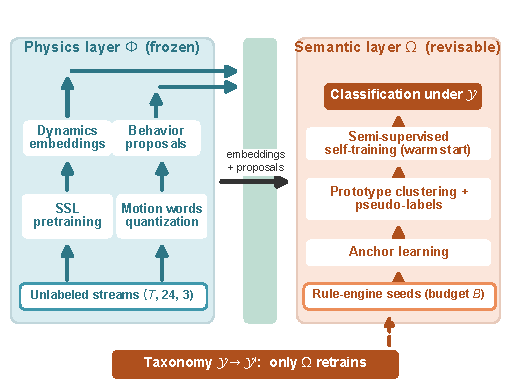
\includegraphics[width=0.76\linewidth]{fig1_framework_overview.pdf}
  \caption{The PSD framework. A frozen physics layer $\Phi$ (left) turns unlabeled skeleton streams into dynamics embeddings and behavior proposals via self-supervised pretraining and motion-word quantization. A revisable semantic layer $\Omega$ (right) expands rule-engine seeds into taxonomy coverage through anchor-guided clustering with iterated confidence-filtered pseudo-labeling, consolidated by self-training and warm-started small-budget initialization. The layers communicate only through embeddings and proposals, so a taxonomy transition $\mathcal{Y}\to\mathcal{Y}'$ retrains $\Omega$ alone.}\label{fig:framework}
\end{figure}
          % hist-draft: introduction.md (Abstract 已内置上方)
% 02-related-work.tex — truth: 本文件（2026-09-10 交割：R22 后全部正文修订直改 tex，原装配源 md 已冻结为历史设计稿，见其头部治理注记）
% 纪律: 三小节主题式 + 每小节 gap 句收尾; tab1 三近邻差距表随行;
% [CITATION-NEEDED] 内嵌标记移除, 作者待补状态记录 refs.bib note(3 条: yolo2025petx/mct2024tip/gra2024tnnls)。
% R3-1/R2-2 修订 (2026-11-15): 新增 §2.4 逐条划界 TREBA/BehaveMAE/ProSL + tab:compmap 失配表;
%   三处 Gap 改写承认动物姿态自监督已有工作; 首次性主张收窄为机制组合级。
% 2026-11-16 回修: §2.4 新增与 class-incremental/continual learning 的定位段（审查#5）,
%   refs.bib 补 rebuffi2017icarl / wang2024continual / masana2023cil 三条经核验题录。

\section{Related work}\label{sec:related}

Animal behavior recognition supports applications ranging from livestock welfare monitoring to working-dog training. Training a single service or assistance dog costs tens of thousands of dollars, and more than half of candidates fail to graduate~\citep{grimm2026science}, which motivates objective, automated behavior assessment. Deployed systems already combine wearable sensors with classical machine learning for canine posture estimation~\citep{plosone2023imu}, yet the field lacks a recognition framework that works when labels are scarce and evaluation criteria keep evolving. We review three bodies of work that bear on this gap---animal behavior understanding, skeleton-based self-supervised learning, and pseudo-label-driven semi-supervised learning---and then position our contribution against the three nearest neighbors and against class-incremental learning (Section~\ref{ssec:rw-position}).

\subsection{Animal behavior understanding}\label{ssec:rw-animal}

Existing animal behavior pipelines divide into appearance-based, pose-based, and sensor-based lines.

Appearance-based methods classify behavior directly from RGB frames or video. YOLO-PetX adapts a detection backbone to anomalous dog behavior~\citep{yolo2025petx}. TP-CanineNet applies temporal contrastive learning with pseudo-labels to canine separation-anxiety video~\citep{tpcanine2025}. These methods inherit the strengths of image recognition but depend on large annotated corpora, and their accuracy degrades under background change, occlusion by handlers, and breed variation in appearance.

Pose-based methods first extract keypoints, then classify dynamics. DeepLabCut~\citep{mathis2018dlc} and SLEAP~\citep{pereira2022sleap} made markerless animal pose estimation practical. Building on such inputs, ASBAR unifies skeleton-based animal action recognition with PoseConv3D and reports 75.3\% top-1 on primate benchmarks~\citep{asbar2024}. BCST-GCN adapts ST-GCN-style graph convolutions with bidirectional cross-attention to pig behavior and reaches 95.36\% average accuracy on its four-behavior dataset compiled from online public videos~\citep{bcstgcn2026}. Hierarchical representation learning of dog behavior from single-view 3D pose has also been explored~\citep{miyai2025workshop}. Skeleton representations are compact, background-invariant, and robust across individuals---properties that should suit low-resource settings---but every behavior classifier above is trained fully supervised on a fixed label set.

Sensor-based methods use accelerometers or IMUs. They capture coarse daily activities reliably~\citep{plosone2023imu} but cannot resolve fine-grained behaviors that differ mainly in body configuration rather than global motion.

\paragraph{Public data landscape.}
The scarcity that motivates this work is visible in the data that actually exists. Among the datasets we could identify, the only large-scale real animal-behavior video benchmark with per-video action labels is Animal Kingdom~\citep{ng2022animalkingdom}, in which dogs appear as a sparsely-labeled subset; canine-specific resources are otherwise wearable inertial time series with ethogram-annotated behaviors~\citep{vehkaoja2022dogsensor,plosone2023imu}, synthetic dog videos built for pose estimation~\citep{shooter2024sydogvideo}, or pose-only still images. To our knowledge none provides real working-dog behavior as skeleton sequences with per-segment expert action labels at benchmark scale. By ``scarce'' we mean skeleton-registered expert behavior labels: Animal Kingdom provides frame-level action labels but no 3D skeletons, so obtaining skeleton sequences requires self-extraction---it is the joint availability of clean skeletons and per-segment action labels, not temporal labels per se, that is missing. Our public-real tier must weakly exploit exactly this, which is why it is assembled by self-extraction from Animal Kingdom (Section~\ref{sec:datasets}) and why the target-domain real-K9 tier is pre-registered yet left unexercised. On our own evidence (Section~\ref{sec:ablation}; the alignment analysis in Section~\ref{sec:conclusion}, L9) the negative end-to-end boundary on the canine tier is attributable to label misalignment and extraction quality in the only public source of canine behavior video with action labels; whether it also reflects true domain-level scarcity is precisely the question the pre-registered K9 pilot is designed to separate.

\paragraph{Gap.}
Current animal pipelines assume a fixed taxonomy and supervision-heavy training. Animal pose self-supervision is no longer unexplored: TREBA learns rodent behavior representations from a fraction of expert labels by programming pretext tasks from domain knowledge~\citep{sun2021treba}, and h/BehaveMAE extends masked autoencoders to spatio-temporal motion-capture sequences, exposing a movement-to-activity hierarchy~\citep{stoffl2024behavemae}. Domain-adaptive pretraining improves primate behavior recognition~\citep{primateda2025}, and self-supervised video pretraining extends to multi-animal settings~\citep{mabe22,beast2025}. What these lines share is that they stop at representations and their evaluation probes: none couples them to temporal behavior proposals, to a label-expansion loop, or to a mechanism for absorbing taxonomy change---no surveyed system is designed so that changing evaluation criteria can be handled without re-annotating the corpus.

\subsection{Skeleton-based self-supervised and unsupervised learning}\label{ssec:rw-ssl}

Self-supervised representation learning for skeletons is mature in the human domain. ST-GCN established graph convolutions over joint topologies~\citep{yan2018stgcn}, and PoseConv3D recasts keypoints as heatmap volumes for 3D convolution~\citep{duan2022posec3d}. Among purely unsupervised objectives, AimCLR maximizes asymmetry across extreme augmented views with an InfoNCE~\citep{vandenoord2018representation} queue~\citep{guo2022aimclr}. Under the linear-evaluation protocol (frozen encoder + FC-softmax classifier; three-stream joint/motion/bone fusion), the conference paper reports 78.9\% on NTU60 cross-subject~\citep{guo2022aimclr}, and the official repository's re-measurement of the released checkpoints gives 79.18\%. Its journal extension is credited with 80.9\% on NTU60 cross-subject linear evaluation in the official repository's results table~\citep{aimclrpp2024}. Cross-view contrastive objectives form a parallel self-supervised family for skeletons~\citep{li2021crossclr}, and we treat the encoder choice as replaceable within our framework; AimCLR serves as the reference physics-layer instantiation rather than a load-bearing design commitment. For temporal structure, unsupervised segmentation methods quantize motion into discrete vocabularies; a motion-word quantization pipeline (SMQ) derives behavior-proposal boundaries from quantized motion-word sequences~\citep{gokay2025smq}.

Two observations motivate our treatment of this literature. First, virtually all benchmarks, augmentations, and graph templates assume the human body plan; transferring these objectives to quadruped kinematics requires adapting joint topology, augmentation priors, and view construction. Second, pretraining and segmentation are studied separately, although a recognition system needs both: representations without proposals cannot localize behaviors, and proposals without semantics cannot name them. State-space backbones such as VideoMamba~\citep{videomamba2024} and Mamba-MSQNet for animal action recognition~\citep{fazzari2024mambamsqnet} offer efficiency alternatives but do not address label scarcity either.

\paragraph{Gap.}
Self-supervised skeleton machinery is mature for humans and, since TREBA and h/BehaveMAE~\citep{sun2021treba,stoffl2024behavemae}, has entered the animal domain---but as representation learning, validated through probes and clustering, and still decoupled from unsupervised temporal decomposition and from any label-expansion loop; our repository-scale survey found no published animal-skeleton pipeline combining self-supervised representation learning with the latter two. In the human skeleton domain, masked autoencoders~\citep{skeletonmae2022} and foundation-model efforts~\citep{skeletonfm2025} pretrain representations for broad downstream transfer; our decoupling claim is orthogonal---the frozen component is the physics encoder, the revisable component is the taxonomy-facing semantic layer, and the measured quantity is taxonomy-transition cost rather than representation quality (systematic repository-scale survey; full matrix in Appendix~\ref{app:novelty}).

\subsection{Semi-supervised, few-shot, and pseudo-label learning}\label{ssec:rw-semi}

Semi-supervised skeleton action recognition in the human domain relies mostly on consistency regularization and teacher--student schemes, including momentum-contrastive teachers~\citep{mct2024tip} and graph-representation alignment~\citep{gra2024tnnls}. These methods regularize predictions under perturbation but receive no external guidance about which classes matter. MAC-Learning introduces anchor-based contrastive learning, where ``anchors'' are contrastive sample pairs selected to structure the embedding space~\citep{mac2022learning}; it does not maintain seed-annotated anchors that supervise cluster assignment, and it includes no iterative pseudo-label loop. Closest in mechanism, ProSL iterates between clustering and pseudo-label generation in self-supervised contrastive learning: starting from a contrastively pretrained encoder, a codebook built by clustering supplies cluster-level pseudo-labels that are progressively refined over rounds~\citep{qin2025prosl}. ProSL targets fully unsupervised representation learning on human benchmarks, whereas PSD runs a \emph{semi-supervised recognition} loop driven by externally supplied rule-engine seed anchors---the semantic layer, not the representation, is the object being trained---and adds confidence filtering, temporal behavior proposals, and the taxonomy-transition cost framing. Point-supervised skeleton action segmentation is another close neighbor: it generates prototype-similarity pseudo-labels with clustering from one labeled frame per segment~\citep{pointsup2026}; our combination differs in rule-engine seed anchors, confidence-filtered iteration, and the taxonomy-transition cost framing---we claim firstness for that combination, not for prototype pseudo-labels per se. Few-shot approaches such as PAINet learn episode-based metric classifiers~\citep{painet2023} and likewise lack a mechanism for expanding labels beyond the support set.

Vision foundation models supply another route to low-shot recognition~\citep{caron2021dino}. Skeleton-to-image encoding maps skeletons into images consumed by VFM-pretrained encoders~\citep{skel2img2026}, demonstrating that foundation-model features transfer to skeleton data. This line uses VFMs for representation only; it does not close the loop from a handful of annotated seeds to full taxonomy coverage. In the animal domain specifically, TP-CanineNet is the closest use of pseudo-labels, operating on RGB video rather than skeletal dynamics~\citep{tpcanine2025}.

\paragraph{Positioning against the nearest neighbors.}
Table~\ref{tab:neighbors} summarizes the nearest neighbors of our semantic-layer design.

\begin{table}[pos=t]
\centering
\caption{Nearest neighbors of the semantic-layer design and their mechanism coverage. None of the surveyed rows couples seed-annotated anchors, cluster-based pseudo-label iteration, and a self-supervised physics encoder for temporal-skeleton recognition.}
\label{tab:neighbors}
\small
\setlength{\tabcolsep}{4pt}
\begin{tabularx}{\linewidth}{p{2.9cm}p{2.0cm}ccc p{1.9cm}}
\hline
Work & Domain & Seed anchors & Cluster + pseudo-iter & SSL enc. & Output \\
\hline
MAC-Learning~\citep{mac2022learning} & Human skel. & $\times$ (pairs) & $\times$ & $\times$ & Repr. \\
ProSL~\citep{qin2025prosl} & Human skel. & $\times$ (clustering) & \checkmark\ (unsuper.) & \checkmark & Repr. \\
Skeleton-to-Image~\citep{skel2img2026} & Skel.\ repr. & $\times$ & $\times$ & \checkmark & Repr. \\
TP-CanineNet~\citep{tpcanine2025} & Canine RGB & $\times$ & Partial & $\times$ & Cls. \\
\textbf{Ours} & \textbf{Quadruped stream} & \checkmark\ (rule-eng.) & \checkmark\ (conf.-filt.) & \checkmark\ (physics) & Recog.+seg. \\
\hline
\end{tabularx}
\end{table}

To the best of our knowledge, transferring the combination of seed-annotated anchor learning, prototype clustering, and iterated confidence-filtered pseudo-labeling to temporal-skeleton recognition has not been reported. Our claim of firstness rests on a repository-scale survey covering ten query groups and eighteen candidate works---twenty-two across the final matrix's eleven rows once the submission-time re-verification row and the revision's three nearest-neighbor rows are included---with zero occupancy (full matrix in Appendix~\ref{app:novelty}), complemented by an arXiv/CrossRef re-verification at submission time that surfaced point-supervised skeleton segmentation~\citep{pointsup2026} as the nearest neighbor---differentiated above and in Section~\ref{ssec:rw-position}. We state this claim for the \emph{mechanism combination}; we do not claim firstness for any individual ingredient (Section~\ref{ssec:rw-position}).

\subsection{Positioning against the three nearest neighbors}\label{ssec:rw-position}

The three nearest neighbors of this work are TREBA~\citep{sun2021treba}, h/BehaveMAE~\citep{stoffl2024behavemae}, and ProSL~\citep{qin2025prosl}. Table~\ref{tab:compmap} maps them, with two further neighbors, against the data and protocol they were built for, and names the specific mismatch that prevents a direct comparison.

\begin{table}[pos=t]
\centering
\caption{Comparability map: nearest neighbors, their data and protocol, and the specific mismatch that prevents a head-to-head comparison with PSD. ``Superv.\ type'' is the supervision signal the method's main result is reported under. None of the rows is directly comparable to our three-tier protocol without re-experimentation, which we therefore do not claim as a comparison.}
\label{tab:compmap}
\small
\setlength{\tabcolsep}{4pt}
\hyphenpenalty=10000
\emergencystretch=1.5em
\begin{tabularx}{\linewidth}{p{2.65cm}p{2.3cm}p{2.3cm}p{1.9cm}X}
\hline
Method & Data / domain & Task \& protocol & Superv.\ type & Protocol mismatch vs.\ ours \\
\hline
TREBA~\citep{sun2021treba} & Mouse fly-courtship / rodent home-cage \textbf{RGB video + pose} & Representation learning; $k$-NN / classification probes, label-efficiency curves & Self-sup. + few expert labels & Image/pose features; no temporal proposals, no semantic layer, no taxonomy-change setting \\
h/BehaveMAE~\citep{stoffl2024behavemae} & Animal mocap (mice, macaques, ASTM) \textbf{pose seqs.} & Unsup.\ masked pretraining; linear probes at three levels & Unsupervised & Pretraining quality only; no recognition pipeline, no pseudo-label loop, no transition-cost view \\
ProSL~\citep{qin2025prosl} & Human skeletons (NTU60/120, Kinetics) & Unsup.\ contrastive learning with iterated cluster pseudo-labels; linear eval & Unsupervised (cluster pseudo-labels) & Trains the \emph{representation}; no seed anchors, no confidence-filtered recognition loop, human-only \\
MAC-Learning~\citep{mac2022learning} & Human skeletons (NTU, Kinetics) & Semi-sup.\ representation learning via anchor contrastive pairs & Partial labels & Anchors = contrastive pairs, not rule-derived seeds; no cluster pseudo-label iteration \\
Point-supervised seg.~\citep{pointsup2026} & Human skeletons & Action segmentation from one labeled frame per segment & Point labels & Single-frame labels, not rule seeds; segmentation only; no frozen-physics decoupling \\
\textbf{Ours (PSD)} & \textbf{Quadruped streams + public human/ape benchmarks} & \textbf{Three-tier pre-registered protocol; recognition + segmentation under taxonomy transitions} & \textbf{Rule-engine seeds (tens of clips)} & --- \\
\hline
\end{tabularx}
\end{table}

\paragraph{TREBA~\citep{sun2021treba} (CVPR 2021).}
\emph{What it does.} Task programming injects domain knowledge into self-supervised pretext tasks (frame--behavior affinity, temporal-order prediction) so that rodent behavior representations can be learned from limited expert annotations; the learned representations are evaluated with $k$-NN and light classifiers, and task programming approaches expert-level labeling efficiency on fly-courtship and mouse home-cage videos. \emph{Where we differ.} TREBA learns an embedding for RGB/pose frames under a fixed ethogram; it has no temporal behavior-proposal stage, no mechanism that converts embeddings into taxonomy-wide labels, and no notion of an evaluation taxonomy that later changes. \emph{PSD increment.} PSD uses its label-free physics layer \emph{as a substrate}: the semantic layer turns embeddings plus unsupervised proposals into labels under the current taxonomy, and the measured quantity is the cost of changing that taxonomy, not probe accuracy.

\paragraph{h/BehaveMAE~\citep{stoffl2024behavemae} (ECCV 2024).}
\emph{What it does.} A hierarchical masked autoencoder for animal motion-capture data (mice, macaques, and the multi-species ASTM benchmark) learns spatio-temporal behavior representations without labels; probes show lower layers encode fine-grained movements and higher layers complex activities. \emph{Where we differ.} h/BehaveMAE is a representation-quality study: its outputs are latents and probe accuracies, not a recognition pipeline. It does not segment continuous streams into behavior proposals, does not expand labels, and does not consider taxonomy evolution. \emph{PSD increment.} PSD treats such encoders as the replaceable frozen physics layer (Section~\ref{ssec:rw-ssl}) and contributes the missing half: a revisable semantic layer and an explicit account of what happens---to accuracy and to wall-clock cost---when the taxonomy changes.

\paragraph{ProSL~\citep{qin2025prosl} (Machine Learning 2025).}
\emph{What it does.} ProSL improves unsupervised skeleton-based action recognition by iterating between clustering and pseudo-label generation: a contrastively pretrained encoder is clustered into a codebook, cluster assignments serve as pseudo-labels, and this loop progressively refines the representation; it reports the strongest published unsupervised results on human skeleton benchmarks. \emph{Where we differ.} ProSL's pseudo-labels are cluster identities used to train the \emph{encoder}; there are no externally supplied seeds, so the label space is the clustering's own---and nothing connects it to a domain taxonomy, to behavior proposals from unsupervised segmentation, or to a transition-cost question. \emph{PSD increment.} PSD inverts the direction of trust: representations are frozen after pretraining, and pseudo-labels grow a \emph{semantic layer} from rule-engine seed anchors toward a prescribed taxonomy under confidence filtering; the evaluated quantities are low-budget recognition accuracy and taxonomy-transition cost. This is also why ProSL cannot be transplanted as a baseline into our three-tier protocol without re-experimentation (Table~\ref{tab:compmap}).

\paragraph{Relation to class-incremental and continual learning.}
Taxonomy evolution under a frozen backbone is adjacent to class-incremental learning (CIL) and continual learning, where a model absorbs new classes over a sequence of tasks without catastrophically forgetting old ones~\citep{rebuffi2017icarl,wang2024continual,masana2023cil}. The two settings share machinery---frozen or slowly updated representations, head re-training, and logit-level reconciliation across label spaces (classifier realignment and logit aggregation for merged heads)---but their objectives differ. CIL methods are designed and benchmarked for incremental accuracy under sequences of disjoint class sets, typically spending rehearsal buffers, distillation, or parameter isolation to resist forgetting~\citep{rebuffi2017icarl,masana2023cil}; PSD asks a different question: the \emph{cost--benefit accounting} of an explicitly declared taxonomy remap $\mathcal{Y}\to\mathcal{Y}'$ over an already-collected unlabeled stream, where the semantic layer rebuilds coverage from rule-engine seeds plus unsupervised proposals and no rehearsal or memory-preservation objective is in play. CIL baselines therefore answer a question our protocol does not ask---accuracy retention across incremental sessions under an arriving-class stream---and are not comparable within our matched-budget, frozen-remap transition protocol without re-experimentation; conversely, our transition-cost endpoints (wall-clock and annotation units at matched accuracy under a frozen remap) are not quantities CIL benchmarks report. We position the two lines as complementary: CIL supplies mechanisms for absorbing \emph{arriving} classes under stability--plasticity trade-offs, while this paper measures when the decoupled structure makes an \emph{arbitrary declared remap}---merges and renames here; splits and additions measured on the synthetic tier (Section~\ref{sec:experiments})---worth absorbing at low cost.

\paragraph{Gap.}
Three absences compound across the three lines reviewed above. Animal behavior understanding offers no label-efficient path and no mechanism for taxonomy change (Section~\ref{ssec:rw-animal}). Skeleton-based self-supervision supplies representation machinery that has begun to reach animals (TREBA, h/BehaveMAE) but stops at representations, and treats segmentation as a separate problem (Section~\ref{ssec:rw-ssl}). Semi-supervised learning supplies pseudo-label machinery---most closely ProSL's cluster-iteration---whose components have, to our knowledge, never been assembled for temporal-skeleton recognition under externally supplied seed anchors (Section~\ref{ssec:rw-semi}). No surveyed method couples a label-free physics layer (self-supervised dynamics modeling plus unsupervised segmentation) with an anchor-guided semantic layer that grows from tens of seeds to a complete, revisable taxonomy. This coupling is the design whose cost--benefit boundary this paper measures.
          % hist-draft: related-work.md (题录池 11 条全解决/3 条作者项已经 CrossRef/arXiv 落库)
% 03-method.tex — truth: 本文件（2026-11-15 深度改造: R3-2/R3-3/R2-4 落实）
%   R3-2: A/P 显式区分 + Eq.(4) 组(原型=类均值、共识门、m_c 频率缩放);
%   R3-3: 种子=高召回低精度先验, 验证流程与标注成本单列, 预算核算口径统一;
%   R2-4: m_c 在 Eq. 组后给最小定义, 完整形式声明见补充材料;
%   AimCLR→SMQ 接口说明入 §3.2.2; SMQ 降级为辅助步骤。
% 纪律: galaxy Method 规范——呈现设计决策, 验证数字留 §4(E1-E6 各段), 此处不重复 Evidence 块;
% fig2 落 §3.3(规格 figure-specs.md, PDF 待绘); Algorithm 1 用 algorithm/algpseudocode.
\section{Method}\label{sec:method}

This section presents the Physics--Semantics Decoupled framework (PSD). Section~\ref{ssec:formulation} fixes notation and gives an overview. Section~\ref{ssec:physics} details the physics layer, which learns \emph{how skeletons move} without any behavior labels. Section~\ref{ssec:semantic} details the semantic layer, which learns \emph{what behaviors are called} from a small seed budget. Section~\ref{ssec:decoupling} formalizes the decoupling mechanism that absorbs evolving evaluation criteria.

\subsection{Problem formulation and overview}\label{ssec:formulation}

\paragraph{Notation.}
Let $X = \{x_1, \dots, x_T\}$ denote an unlabeled skeleton stream, where $x_t \in \mathbb{R}^{J \times 3}$ holds 3D joint coordinates for $J$ joints at frame $t$. A taxonomy $\mathcal{Y}$ maps behavior names to labels; evaluation criteria evolve by replacing $\mathcal{Y}$ with $\mathcal{Y}'$. The annotation budget is a set $S$ of seed clips with coarse labels produced by a rule engine over physical priors; $U$ denotes the unlabeled proposal set, $P$ the prototype set, and $B$ the human-annotation budget in clips consumed by the queue. We write $A = \{(e_i, \tilde{y}_i)\}_{i=1}^{N_A}$ for the \emph{seed anchors}---physics-layer embeddings $e_i = \Phi(s_i)$ of seed segments $s_i \in S$ carrying rule-engine coarse labels $\tilde{y}_i$---and reserve $P = \{(\mu_c, y_c)\}$ for the \emph{class prototypes}; the two are distinct objects (Section~\ref{ssec:proto}).

\paragraph{Framework overview.}
PSD factorizes recognition into two layers with a narrow interface. The \emph{physics layer} $\Phi$ maps skeleton windows to dynamics embeddings, trained once per species family on unlabeled streams; it comprises self-supervised pretraining (Section~\ref{ssec:pretrain}) and unsupervised temporal segmentation (Section~\ref{ssec:segmentation}). The \emph{semantic layer} $\Omega$ maps dynamics embeddings and segment proposals to labels under the current taxonomy $\mathcal{Y}$; it comprises seed-anchor construction (Section~\ref{ssec:anchors}), prototype clustering with iterated pseudo-labeling (Section~\ref{ssec:proto}), and semi-supervised self-training with small-budget initialization (Section~\ref{ssec:selftrain}). The layers interact only through embeddings and proposals. This constraint is what allows $\mathcal{Y} \to \mathcal{Y}'$ transitions to leave $\Phi$ untouched (Section~\ref{ssec:decoupling}).

\subsection{Physics layer}\label{ssec:physics}

\subsubsection{Self-supervised pretraining}\label{ssec:pretrain}

We adapt extreme-asymmetry contrastive pretraining~\citep{guo2022aimclr} to quadruped skeletons. Three adaptations matter. First, the joint graph is rebuilt for the target species topology rather than the human body plan; our pipeline uses a 24-joint quadruped layout mapped into an NTU-compatible view via an identity correspondence plus one dead slot. Second, augmentation primitives are restricted to transformations that preserve quadruped plausibility. Third, the official weight initialization is deliberately skipped: re-initializing all convolutional and linear weights to $\mathcal{N}(0, 0.02)$ collapses representations into a cone from which InfoNCE cannot escape on our data, and skipping it restores normal convergence. We report this as a reproducibility note for practitioners reusing official code bases.

\subsubsection{Unsupervised temporal segmentation}\label{ssec:segmentation}

Continuous skeleton streams must be cut into behavior-proposal units before labeling. We use motion-word quantization~\citep{gokay2025smq} as an \emph{auxiliary front-end}, not as a contribution claim: local motion patterns are quantized into a discrete vocabulary, and segment boundaries are proposed where the quantized sequence changes regime.

\paragraph{Interface to the physics encoder.}
SMQ consumes the same species-adapted skeleton view that the physics layer is trained on---SMAL-native 24-joint coordinates resampled to a fixed window---rather than the NTU-compatible 25-slot view used inside AimCLR; a dedicated adapter performs the view conversion, so the two components share data provenance but neither consumes the other's internal representations. On the embedding side, SMQ delivers only segment boundaries: every proposal is then encoded by the \emph{frozen} $\Phi$ into a dynamics embedding (the same features the semantic layer consumes), and no SMQ-internal codebook or quantizer state enters $\Omega$. The interface is therefore exactly ``(boundaries in, $\Phi$-embeddings out)'', which keeps the segmentation module replaceable---Section~\ref{sec:ablation} ablates SMQ against uniform-window and fixed-grid alternatives under this same interface, and reports the comparison honestly: on the small public-real evaluation suite SMQ's boundary IoU is statistically on par with a fixed-grid probe, so the segmentation choice is a measured operating decision rather than a load-bearing component of our claims.

\subsection{Semantic layer}\label{ssec:semantic}

The semantic layer grows labeled coverage toward completeness of the taxonomy from the rule-engine seed set $S$, following the anchor--cluster--pseudo-label recipe transferred from image-domain few-shot recognition~\citep{snell2017prototypical} (Section~\ref{ssec:rw-semi}).

The transfer required re-engineering, not re-application, because three domain shifts bind: First, anchors must be defined over \emph{temporal segment embeddings} from a self-supervised physics encoder instead of image features, so anchor quality depends on representation adequacy (Section~\ref{ssec:pretrain}). Second, prototype clustering operates on variable-length proposals delivered by unsupervised segmentation rather than fixed-size inputs, coupling label-expansion quality to segmentation quality (Section~\ref{ssec:segmentation}). Third, confidence calibration must tolerate quadruped kinematics whose intra-class motion variance differs from both image textures and human locomotion. Each shift is validated separately in Sections~\ref{sec:experiments}--\ref{sec:ablation} before the composed pipeline is evaluated.

\subsubsection{Seed anchors and their verification}\label{ssec:anchors}

Rule-engine coarse labels over physical priors provide seed anchors $A = \{(e_i, \tilde{y}_i)\}$, where $e_i$ are physics-layer embeddings of seed segments and $\tilde{y}_i$ are the engine's coarse labels. Anchors are the \emph{only} labeled objects the loop consumes; unlike anchor-based contrastive objectives that treat anchors as sample pairs~\citep{mac2022learning}, our anchors carry semantic identity and directly supervise cluster assignment.

\paragraph{Seeds are priors, not ground truth.}
The rule engine is deliberately tuned for high recall at the cost of precision: it triggers on physical priors (paw-height ordering for gait classes, head-cluster height for posture classes) and emits a per-segment confidence from rule margin, with short ambiguous spans merged into high-confidence neighbors. We therefore treat every seed label $\tilde{y}_i$ as a noisy prior, never as ground truth, in three concrete ways. (1)~\emph{Quality gating at ingestion}: seed segments enter $A$ only if the engine's own confidence is at least $0.8$ and the segment spans at least $0.5$\,s; segments labeled \emph{unknown} are discarded. (2)~\emph{Verification before write-back}: only seed labels that survive a human spot-check enter the verified anchor set used by the consolidation step (Section~\ref{ssec:selftrain}); unverified seeds supervise only the expansion loop, whose confidence gate is calibrated to tolerate their noise. (3)~\emph{Noise robustness by construction}: anchors initialized from noisy seeds are corrected by confidence-filtered cluster consensus and audited in downstream evaluation (Section~\ref{sec:ablation} reports the seed-noise injection study) rather than trusted as ground truth.

\paragraph{What seed verification costs.}
The verification budget is part of the annotation accounting and is never free. Concretely, verifying one seed clip means a human auditor watches the segment and confirms or corrects its coarse label---a binary decision per segment, an order of magnitude cheaper than full frame-level annotation of the same clip, which requires marking onset and offset of every behavior. Under the loop's accounting, the effective supervision budget is therefore $|S_{\mathrm{verified}}| + |S_{\mathrm{unverified}}| \cdot c_{\mathrm{spot}} + B$ clips-equivalents, where $c_{\mathrm{spot}} \ll 1$ is the per-clip spot-check cost in units of full clip annotations and $B$ is the low-confidence queue budget of Section~\ref{ssec:proto}. We report annotation units in this caliber throughout, and the seed clips consumed by the warm-start initialization of Section~\ref{ssec:selftrain} are counted inside $|S|$, not in addition to it: warm-starting reuses \emph{already-verified} source-domain anchors, so it adds no new seed cost---the remaining marginal cost of adaptation is the $B$ (or, at minimum, 20-clip) offset-domain budget, which is how the budget curves of Section~\ref{sec:experiments} are read.

\subsubsection{Prototype clustering and iterated pseudo-labeling}\label{ssec:proto}

\paragraph{Anchors versus prototypes.}
Seed anchors $A$ and class prototypes $P$ are different objects with different roles, and conflating them is precisely the confusion this subsection removes. Anchors are \emph{labeled exemplar embeddings}: a fixed set of (embedding, coarse-label) pairs produced by the rule engine, consumed as supervision, and never re-estimated. Prototypes are \emph{class-representative vectors}: one per taxonomy class under the current round's labeling state, maintained as free parameters of $\Omega$ and re-estimated every round. A prototype is always the \emph{class mean} of the labeled support it represents: given the currently labeled set (verified seeds plus the confidence-filtered pseudo-labeled pool), the prototype of class $c$ is
\begin{equation}\label{eq:proto}
\mu_c \;=\; \frac{\sum_{i \in \mathcal{I}_c} \phi(e_i)}{\bigl\lVert \sum_{i \in \mathcal{I}_c} \phi(e_i) \bigr\rVert_2}, \qquad \mathcal{I}_c = \{\, i : \text{$i$ labeled as $c$ in the current round} \,\},
\end{equation}
where $\phi(\cdot)$ denotes $\ell_2$ normalization; i.e., the mean of the support members' normalized embeddings, re-normalized. Initially $\mathcal{I}_c$ contains only seed anchors with $\tilde{y}_i = c$; as pseudo-labels accumulate, pool members join $\mathcal{I}_c$ and $\mu_c$ tracks the class mean of the union. This update rule is deliberately the plain class mean---no momentum, no learned projection---so that prototype drift is fully attributable to the labeled-set composition, which the stopping rule of Algorithm~\ref{alg:pseudoloop} monitors.

\paragraph{Assignment, consensus, and admission.}
Unlabeled proposals from Section~\ref{ssec:segmentation} are embedded by $\Phi$ and assigned by the current classifier $\Omega$ (the \emph{head path}); the prototype path provides a second opinion. Writing $\hat{y}_u^{\Omega}$ for the head's prediction, $p^{(1)}_u \geq p^{(2)}_u$ for its top-1 and top-2 class posteriors, and $\hat{y}_u^{P}$ for the nearest-prototype prediction $\arg\max_c \phi(\Phi(u))^{\top} \mu_c$, a proposal $u$ is admitted to the pseudo-label pool only if
\begin{equation}\label{eq:pool}
\underbrace{\hat{y}_u^{\Omega} = \hat{y}_u^{P}}_{\text{prototype consensus}} \;\wedge\; \underbrace{\kappa(u) \,\geq\, \tau_{\hat{y}_u^{\Omega}}}_{\text{calibrated margin gate}}, \qquad \kappa(u) = \frac{p^{(1)}_u - p^{(2)}_u}{m_{\hat{y}_u^{\Omega}}},
\end{equation}
where $\kappa(u)$ is the calibrated top1$-$top2 margin. The consensus condition is governed by the designated high-error seed class in the physics-prior label space (the standing posture in our instantiation); on tiers whose taxonomy lacks that class it degenerates to the margin gate alone, and nearest-prototype assignment is the ablated fallback configuration. Proposals passing Eq.~\eqref{eq:pool} receive pseudo-labels; the pool is re-filtered each round (replacement, not monotone accumulation); prototypes are then re-estimated by Eq.~\eqref{eq:proto}. Figure~\ref{fig:pseudoloop} depicts the loop and Algorithm~\ref{alg:pseudoloop} summarizes it.

\paragraph{Class-specific thresholds and $m_c$.}
The operating threshold $\tau$ is fixed once by quantile targeting on estimated coverage at the first round (the same $\tau$ is reused in every later round to prevent drift), and each class receives a scaled threshold
\begin{equation}\label{eq:mc}
\tau_c \;=\; \tau \cdot m_c, \qquad m_c = f\!\left(\pi_c / \pi_{\max}\right),
\end{equation}
where $m_c$ is a \emph{frequency-aware scaling factor} built from the ratio of class $c$'s seed prior $\pi_c$ to the largest class prior $\pi_{\max}$: rare classes receive $m_c \leq 1$ (a lower admission bar, countering long-tail suppression), majority classes receive $m_c \approx 1$, and a floor prevents the bar from collapsing on extreme tails. The concrete functional form of $f(\cdot)$ and its sensitivity parameters (exponent and floor ratio) are hyperparameters of the protocol rather than tuned per benchmark; we state the required shape here and give the exact instantiation, default values, and ablation hooks in the supplementary material.

\begin{figure}[pos=tbp]
  \centering
  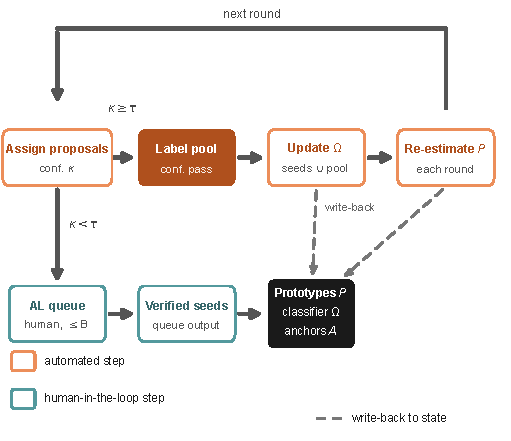
\includegraphics[width=\linewidth]{fig2_pseudo_label_loop.pdf}
  \caption{The anchor-guided pseudo-labeling loop as a two-row pipeline around a shared state hub. Automated loop (top row, left to right): Assign proposals applies the consensus-and-margin gate of Eq.~\eqref{eq:pool} ($\hat{y}^{\Omega}_u = \hat{y}^{P}_u$ and $\kappa(u) \geq \tau_{\hat{y}^{\Omega}_u}$) to route admitted proposals into the label pool; $\Omega$ is updated on verified seeds $\cup$ pool, prototypes are re-estimated by the class-mean update of Eq.~\eqref{eq:proto}, and the next round returns to Assign along the top. Human branch (bottom row): low-confidence proposals ($\kappa < \tau$) divert to an annotation queue (budget $B$ of 100--200 clips); verified seeds write back to the anchor set $A$. The dark hub carries the shared state ($P$, $\Omega$, $A$) that the dashed write-back spokes update each pass; the physics encoder $\Phi$ remains frozen throughout (not shown). Orange-labeled steps are automated; teal-labeled steps are human-in-the-loop. The annotation queue is a deployment extension of Algorithm~\ref{alg:pseudoloop}.}\label{fig:pseudoloop}
\end{figure}

\begin{algorithm}[t]
\caption{Anchor-guided iterative pseudo-labeling}\label{alg:pseudoloop}
\begin{algorithmic}[1]
\Require physics encoder $\Phi$ (frozen), seed anchors $A$, unlabeled proposals $U$, threshold $\tau$, margins $m_c$
\Ensure classifier $\Omega$ under taxonomy $\mathcal{Y}$
\State initialize prototypes $P$ as class means of $A$ (Eq.~\eqref{eq:proto})
\Repeat
  \State assign each $u \in U$ via $\Omega$; prototype opinion $\hat{y}^{P}_u$; confidence $\kappa(u)$
  \State $L_{\mathrm{high}} \leftarrow \{u : \hat{y}^{\Omega}_u = \hat{y}^{P}_u \wedge \kappa(u) \geq \tau_{\hat{y}^{\Omega}_u}\}$ (Eq.~\eqref{eq:pool}); re-filter the pseudo-labeled pool (replacement)
  \State update $\Omega$ on verified seeds $\cup$ pseudo-labeled pool
  \State re-estimate $P$ as class means of the labeled set (Eq.~\eqref{eq:proto})
\Until{proposal assignment stabilizes, the iteration budget is reached, or (where a rule-derived consensus reference exists) pool precision against it drops for two consecutive rounds}
\end{algorithmic}
\end{algorithm}

Design decisions fixed at this stage: confidence filtering uses calibrated classifier margins divided by the class margin scale $m_c$ (prototype margins in the fallback path); each iteration retrains only $\Omega$, never $\Phi$; the iteration budget guards against confirmation bias accumulating across rounds; and seed-noise amplification is bounded by the three-part seed treatment of Section~\ref{ssec:anchors} (ingestion gating, spot-check verification before write-back, and consensus correction), so rule-engine seeds act as high-recall/low-precision priors rather than ground truth. The precision-drop stopping rule monitors pool precision against the physics-prior consensus reference---a weak, rule-derived proxy rather than human annotation. On tiers where training-split labels are fully observed but no rule-derived consensus exists (the Animal Kingdom and NTU end-to-end arms), the rule is disabled and iteration stops on convergence or the iteration budget; the consolidated classifier consumes verified seed labels plus pseudo-labels for pool clips, never pool ground truth. Class imbalance in animal behavior distributions (long-tail rare behaviors) is handled at the prototype level via the frequency-aware thresholds of Eq.~\eqref{eq:mc} rather than resampling; a head-to-head ablation of this choice (margins vs.\ resampling vs.\ no handling) is registered for the public-real tier and not yet run (Section~\ref{sec:ablation}, Sensitivity). The consensus condition of Eq.~\eqref{eq:pool} governs a designated high-error seed class (the standing posture in the physics-prior label space); on tiers whose taxonomy lacks that class (the Animal Kingdom and NTU class spaces) it passes all proposals by construction.

\subsubsection{Semi-supervised self-training and small-budget initialization}\label{ssec:selftrain}

Pseudo-labeled coverage is consolidated by iterative retraining of $\Omega$ on the growing pool---pool clips enter with their pseudo-labels, and only \emph{verified} seed clips contribute ground-truth labels---in the semi-supervised self-training tradition motivated by TCL~\citep{singh2021tcl} (whose temporal-contrastive consolidation step is not used here). To make very small annotation budgets usable, a warm-start protocol initializes small-budget training from the semantic-layer weights of a full-budget model trained on the same taxonomy under the noise-offset protocol of Section~\ref{sec:experiments}, before expansion proceeds within the budget $B$. Warm-starting is a transfer of \emph{verified} source-domain anchors and semantic-layer weights, so it consumes no new seed budget; the total supervision accounting (verified seeds, spot-check effort, and the target-domain budget) follows Section~\ref{ssec:anchors}. Figure~\ref{fig:pseudoloop} illustrates the complete loop.

\subsection{Decoupling mechanism}\label{ssec:decoupling}

We formalize an evaluation-criteria evolution as a taxonomy transition $\mathcal{Y} \to \mathcal{Y}'$ (splitting, merging, renaming, or adding behaviors). We report the transition cost $C(\mathcal{Y} \to \mathcal{Y}')$ as a pair---human annotation units consumed and wall-clock retraining time---kept in separate units rather than summed, measured at matched final accuracy. Under decoupling: (1) the physics layer $\Phi$ and its pretrained parameters remain frozen; (2) existing segment proposals are re-used---only their label assignments change; (3) the semantic layer is rebuilt through Section~\ref{ssec:semantic} using seeds under $\mathcal{Y}'$; and (4) the reported quantity is $C_{\mathrm{decoupled}}(\mathcal{Y} \to \mathcal{Y}')$ versus $C_{\mathrm{full}}(\mathcal{Y} \to \mathcal{Y}')$, where the full baseline retrains representation learning under $\mathcal{Y}'$. We hypothesize that $C_{\mathrm{decoupled}} < C_{\mathrm{full}}$ at matched accuracy, and that accuracy under $\mathcal{Y}'$ matches full retraining within noise; Section~\ref{sec:experiments} (E6) tests both hypotheses.
                % hist-draft: method.md
% 04-experiments.tex — truth: 本文件（2026-09-10 交割：R22 后全部正文修订直改 tex，原装配源 md 已冻结为历史设计稿，见其头部治理注记）
% 纪律: 4.1 数据集与三层口径协议(20/24 有效监督口径随行) / 4.2 实现细节+统计协议 / 4.3 主实验 E1-E6(每实验先声明 claim 句) /
% 4.4 对比研究(NTU 等价性段=成文块装配); tab2 真实 K9 列空缺如实标注; 内部路径/文件名禁入正文(ROUND2 发现#7)。
% 2026-11-16 回修（审查#3/#4/#11/#12）: 归因对照补 episode/budget 口径披露（60→10 界 vs 60→49 复制; 50/class 三臂 vs E6 n=30/100）;
%   E6 正文标注 n=3; tab:main caption 注明合成层全预算参照为单 run。逐 seed 配对比值入 supplementary (app:e6seeds)。
% 2026-11-16 P1 收官补位（写手·补充细节）: E1 同 episode（60→49）零重训界结果位预留（ssec:boundary 界段改为已注册待测
%   + tab:attribution-controls 增 60→49 界两行, \TODO 待回填）; E2/E3 协议与数字位、CIL 定位段入 supplementary
%   （app:mergebound49 / app:rebuildbudget / app:synthmigration / app:cil）。数字位禁编造, 由回填写手按实验产物回填。
% 2026-11-16 P1 回填（回填写手）: E1/E2/E3 出数, 数字源 runs/p1_sprint/{zerobound_6049,semantic_rebuild_1100,
%   split_addition_episode}/summary.json（reports/p1_sprint_evidence/ 有逐字节一致副本）——
%   tab:attribution-controls 60→49 界两行（68.04/67.97）与 E2 等预算三臂行（D′ 60.2% vs C′ 44.9%, 26.5×）已回填;
%   ssec:boundary/E6/E6-real-2 同步改"已测"; 60→10 与 60→49 两个 episode 不可互换的口径说明已强化。
% 2026-11-16 统稿: 新增 Reinforcement E3（split/addition 残余价值探测）与 E3b（k∈{10,25,50,100} 标注预算阶梯）
%   正文段 + tab:kladder——摘要/贡献1/结论所引 k 阶梯实验的正文载体; 协议全文在 supplementary app:synthmigration/app:kladder。
%   数字源 runs/p1_sprint/{split_addition_episode,k_ladder}/summary.json（reports/p1_sprint_evidence/ 有镜像）, 禁编造。
% 2026-11-16 P1 真实 tier 冻结编码器对照（统稿）: ssec:boundary 冻结对照 bullet 由"未运行/不赋值"改为已执行结果
%   （NTU120/UCF101/PanAf500 三臂 C/A/B；NTU60 未重跑, 沿用已报告 E9 参照 67.53±0.24）, tab:attribution-controls
%   增真实 tier 十行块, caption 同步; 协议全文在 supplementary app:frozenreal。数字源 runs/p1_sprint/{ntu120,ucf101,
%   panaf500}/summary.json, 与 reports/p5b-ntu120|p5b-ucf101|p23-panaf-retention-2026-09-07.json 逐位一致, 禁编造。
% 2026-11-16 终审回修（回修写手）: E9b/E9c 段补基准口径披露（NTU120=12,000-clip/60 类子集、UCF101=10,000-clip 子集,
%   各臂同口径; UCF101 官方 split1 val 仅 463 clips 一并注明）; tab:attribution-controls 表注同步 subset calibers
%   + 真实 tier 块无端到端微调臂的限定（frozen-vs-full-FT 对照仅合成层证据）; E3 decoupled 均值 45.8%→45.7%（三种子
%   0.4448/0.4345/0.4931 均值 0.45747 直接舍入, 消除两级舍入）。
% 2026-11-16 P1 头对头回填（写手·结果回填）: sec:comparison 新增 published-method 基线段 + tab:h2h——
%   AimCLR 线性评测（joint stream, 官方 LE recipe, in-house pretext 权重）10%/full = 66.71/74.30%,
%   监督 ST-GCN（端到端, 16 hidden channels, 0.84M 参数）10%/full = 66.52/83.46%, 与 E9 的 PSD 臂
%   （linear head 66.05 / semantic 67.53±0.24 / full 参照 74.45）同 10% 分层子集（seed 42, 4,009 clips）、
%   同 40,091 全量、同 16,487 验证集并排; 基线臂为单 run, 10% 差距仅作描述不下显著性结论。
%   数字源 runs/p1_sprint/{published_baseline_ntu60,supervised_stgcn_ntu60}/summary.json, 禁编造。
% 2026-11-16 P1 k 阶梯多种子回填: k=10/25/50 档补 seeds 43/44（同日补测, 初测单种子 readout 与合并三种子 summary 均存档）,
%   decoupled 45.29±0.16 / 59.08±2.52 / 65.06±1.33 / 72.41±0.00%（k=10/25/50/100, std ddof=0）,
%   边际 50.57/36.78/30.80/23.45pp; 数字源 runs/p1_sprint/k_ladder/summary.json（canonical 合并版）, 禁编造。
\section{Experiments}\label{sec:experiments}

\subsection{Datasets and the three-tier protocol}\label{sec:datasets}

Because no available dataset spans the scenarios our claims require (Section~\ref{ssec:rw-animal}), we evaluate under a three-tier protocol; numbers are never mixed within a comparison. The \emph{synthetic} tier serves pipeline shake-down and controlled ablations; the \emph{public-real} tier provides label-free and low-resource evaluation on real animal skeletons; the \emph{real-K9} tier (working-dog training footage) is reserved for the target domain and is not exercised in this study. Two further contexts are exercised under the same reporting rules and never pooled with the tiers: a \emph{synthetic-offset} variant of the synthetic tier (the same generator with Gaussian joint-coordinate noise, $\sigma{=}0.10$; its distribution fixed by a pre-registered diagnostic before any offset experiment ran) for the distribution-shift and warm-start studies, and public \emph{benchmarks} (NTU60/NTU120/UCF101 for human actions and PanAf500 for great apes) for the pre-registered E9-series cross-domain retention studies, each reported against its own full-budget reference. The working-dog pilot is nonetheless pre-registered before any data collection (protocol PSD-K9-PREREG-001, committed to the public review repository): a double-annotation agreement gate (Cohen's $\kappa\geq 0.60$), session-level splits, a single primary endpoint with a paired decision rule, and a no-redistribution clause for raw footage and derived skeletons.

The public-real tier draws on three sources. InterPet4D~\citep{peng2026interpet4d} provides 226 SMAL-fitted skeleton sequences of human--pet interactions (225 used; one all-NaN sequence excluded and listed) as the unlabeled stream for self-supervised pretraining and segmentation evaluation. From the official Animal Kingdom action-recognition lists~\citep{ng2022animalkingdom} we aggregate the canine-species subset: 329 videos (231 train / 98 test) with 34{,}772 frame-level annotation rows, for weak-supervision and behavior-classification evaluation. APTv2~\citep{yang2023aptv2} supplies a large pose pool (official: 2{,}749 clips, 41{,}235 frames; local inventory 41{,}179 images; consumed unlabeled) for expansion experiments. Skeletons are world-coordinate keypoint sequences of shape $T{\times}24{\times}3$ with a per-joint confidence channel. One structural caveat applies to every real-domain skeleton product: the dog-pose annotations never label four of the 24 graph slots (both eyes, withers, throat), so real-domain keypoints are topology-isomorphic with 20/24 effective supervision channels; the four dead channels are hard-masked at assembly and NaN-guarded downstream. A pre-registered expansion tier (v2; PSD-AKV2-PREREG-001, frozen before the build) re-extracts the same canine videos as multiple contiguous segments under a per-frame label-consistency gate, yielding 352 clips in an eight-class space; it serves as a parallel replication layer and never replaces v1 numbers (E7b).

\subsection{Implementation details}\label{sec:implementation}

All experiments run on a single consumer GPU (RTX 5060 Laptop, 8\,GB); self-supervised pretraining takes about 13 minutes for 120 epochs on InterPet4D, so the physics layer is reproducible without data-center resources. Pretraining uses a learning rate of 0.05, a queue of 1{,}024, and window length $T{=}64$; this is the first working setting, not the outcome of a systematic search. $k$-NN probes report 5-fold mean$\pm$std; end-to-end arms report seed-level dispersion (sample std, ddof~1), not confidence intervals; per-experiment seed choices are listed in the released experiment ledger and protocol files. Aggregate comparisons carry paired seed-level tests with Holm--Bonferroni correction within each experiment family (corrected values printed alongside), effect sizes with a random-baseline reference, and outliers explained rather than removed. The E9-series correction family (Section~\ref{sec:comparison}) consolidates eight paired tests: the pipeline-versus-linear gap tests on three tiers (NTU60, NTU120, UCF101; one-sample $t$ and Wilcoxon signed-rank each) plus the two external-SSL Wilcoxon tests. Each member's decision rule was fixed by its own pre-registered protocol before its run; the consolidated family was fixed before corrected inference entered this manuscript (dated 2026-09-07 in the repository). The PanAf500 gap is reported directionally and is not a family member (its arm distribution ties with the linear arm; raw $p=0.75$); adding it as a ninth member changes no corrected verdict, and under the narrower six-test gap-only sub-family every qualitative conclusion is unchanged. The head-to-head significance tests against the two published-method baselines (Table~\ref{tab:h2h}) are a separate post-hoc two-test family added in this revision (dated 2026-11-16/17 in the repository; per comparison, Welch is the primary test and Mann--Whitney the distribution-free sensitivity analysis, both Holm-corrected within the two-test family: the AimCLR gap reads raw $p{=}1.1\times10^{-6}$ Welch / $6.7\times10^{-4}$ Mann--Whitney, corrected $p{=}2.3\times10^{-6}$ / $1.3\times10^{-3}$); they are not members of the pre-registered E9-series family, and either family choice leaves the reported conclusions unchanged. Registration fixes decision rules before outcomes exist and prevents selective reporting; it did not catch the protocol-implementation errors we corrected (the oracle-label leakage of the initial end-to-end runs, Section~\ref{ssec:proto}), which came from internal adversarial review. Protocol freeze is evidenced by the dated commit history of the public review repository (tag \texttt{review-snapshot}); one protocol (the v2 expansion) and its results landed in the same repository batch, so its freeze is bookkeeping-grade evidence rather than third-party timestamping.

\subsection{Main results}\label{sec:main-results}

Table~\ref{tab:main} consolidates the main results across the three tiers plus the public human-domain benchmark used for implementation-equivalence verification; each numbered experiment below opens by stating the claim it tests; experiment labels follow the released experiment ledger (E5, the active-learning study, is reported as an exploratory finding in Section~\ref{sec:ablation}; E8, the budget curve, is folded into the E7 discussion). Claim tags: \textbf{C1} decoupled transition cost, \textbf{C3} pretraining value, \textbf{C4} unsupervised segmentation, \textbf{C5} anchor-guided semantic expansion, \textbf{C6} low-budget self-training behavior, \textbf{C7} active learning (exploratory negative); \textbf{C2} is the novelty claim, tested by the survey (supplementary material, Novelty survey matrix) rather than by an experiment.

\paragraph{E1: representation quality of the physics layer (C3).}
This experiment tests whether self-supervised pretraining on unlabeled quadruped skeletons yields discriminative dynamics representations. Using subject identity as a $k$-NN probe on InterPet4D (a proxy task that measures representation discriminability, not behavior accuracy), pretraining reaches \textbf{20.89\% $\pm$ 4.04\%} top-1 (sample std over the five folds) against an 8.33\% random baseline ($2.51\times$). The fold-level range is wide (15.56--26.67\%), attributed to the small number of sequences and subject diversity; a projection-head feature caliber yields 12.89\% ($1.55\times$), recorded in the released run report, and both calibers are valid views of the same encoder.

\paragraph{E2: unsupervised segmentation quality (C4).}
This experiment tests whether motion-word quantization cuts continuous streams into behavior-aligned proposals. Under a seeds pseudo-ground-truth protocol, boundary IoU against held-out annotations is \textbf{0.458 $\pm$ 0.049}, versus an equal-segment-count random-cut null of 0.323 $\pm$ 0.022 (Monte-Carlo expectation over 200 random cuts); boundary F1 is reported alongside (0.343 vs.\ the uniform-window 0.396), and the fixed-grid probe that is statistically on par with SMQ ($0.453 \pm 0.027$) is reported in Section~\ref{sec:ablation}.

Figure~1 of the supplementary material visualizes the resulting boundaries against the seed pseudo-ground-truth on the lowest- and highest-IoU episodes.

\paragraph{E3: anchor-guided label expansion (C5).}
This experiment tests whether a small rule-engine seed set expands toward taxonomy coverage via iterated pseudo-labeling. Anchor-guided prototype clustering reaches purity \textbf{0.5339} against a 0.3306 random-assignment baseline ($1.61\times$) and a 0.4858 all-majority baseline ($+4.8$\,pp; the binding comparison). Injecting 30\% label noise into the seeds degrades purity by only 3.1\,pp (0.5025$\pm$ 0.0063, still $1.52\times$ baseline), and enlarging the seed ratio from 25\% to 100\% changes purity by less than 1\,pp at $K\in\{5,10\}$ but costs 2.4\,pp at $K{=}14$, the best cell of the $k$-means sensitivity sweep (the main run is the deterministic class-mean configuration; full sweep in the released evidence archive). Prototype quality saturates early in seed ratio at small $K$, which is what makes a small seed budget practical.

\paragraph{E4: semi-supervised self-training on the public-real tier (C6).}
This experiment tests whether self-training converts pseudo-labeled coverage into usable classification under scarce labels. Iterating from round~0 to round~1 raises pseudo-label pool precision from 0.5125 to \textbf{0.691 $\pm$ 0.013} (a $+17.9$\,pp endpoint gain; the paired first-to-last statistic over all iterated rounds is $\Delta$ $+10.69\pm3.28$\,pp; the two numbers measure different spans and are both released); the precision-drop stopping rule fired after two consecutive degraded rounds, so round~1 is the reported operating point (Holm-corrected $p=0.090$ over the three-test family: the calibrated main first-to-last test, its no-consensus ablation, and the $\alpha{=}0$ control; released artifact \texttt{r16-holm-p04}; raw $p=0.030$, direction-consistent but not significant after family correction). Under the pre-registered partial-class protocol on the Animal Kingdom canine subset (4 of 12 classes pass the sample-size gate), a frozen-backbone classifier with a re-trained head reaches 41.5\% $\pm$ 5.9\,pp overall across three seeds (best seed 44.90\%), $1.66\times$ the 25\% uniform-random baseline ($1.80\times$ at the best seed). The per-class breakdown (watch 100\% / track 23.5\% / jump 0\% / stay 0\%) accompanies this number: the aggregate is dominated by class imbalance and interprets only in the four-class partial caliber (other public-real results carry their own class-space labels).

\paragraph{E7: end-to-end pipeline at small budget (C6; negative boundary).}
This experiment tests whether the complete pipeline, run end-to-end from a small annotation budget, approaches full supervision; it is the paper's principal negative boundary: on the only truly animal target domain exercised end-to-end (canine), the pipeline does not beat chance or a generic-SSL control (mechanism analysis in Section~\ref{ssec:boundary}). The arms follow a corrected protocol (revision R16 of the repository's experiment ledger): the final classifier is trained on seed ground-truth labels plus pseudo-labels for the confidence-filtered pool clips (never on pool ground truth), and iteration stops on convergence or the iteration budget (the precision-drop rule monitors pool precision against a rule-derived consensus reference, which this tier's label space does not provide; consuming true labels there would be oracle leakage; Section~\ref{ssec:proto}). On the 12-class-protocol public-real tier (9 classes with samples; 197 self-extracted clips; anchors and pool restricted to the training split, validation isolated), at 2 clips per class (18 of 141 training clips, $\approx$13\%; ten seeds) the pipeline reaches \textbf{9.8\% $\pm$ 7.5} top-1, at the tier's 11.1\% chance level, against 33.93\% under full supervision; the generic-SSL control reaches 15.2\% $\pm$ 5.1 and the scratch control 8.4\% $\pm$ 10.7; after per-tier Holm correction the only significant same-seed effects are on macro-F1, both favoring the generic-SSL arm ($5.1$\,pp at 2 clips/class, corrected $p=0.023$; $6.6$\,pp at 4, corrected $p=0.049$); warm-versus-scratch differences are not significant. The prototype-path consensus gate is inert on this taxonomy (no standing class; Section~\ref{ssec:proto}), so pool filtering reduces to the confidence margin alone. The iterated pseudo-labeling is the point of failure: pool pseudo-label precision, measured post hoc against training-split labels as a released diagnostic only, averages 0.11 across seeds, and a ground-truth-free per-round recalibration of the gate does not rescue it ($8.9$--$12.5\%$, three seeds). The negative boundary\footnote{An earlier internal protocol variant trained the final head on the pool clips' ground-truth labels and consumed oracle precision for stopping; its higher low-budget numbers were never published and are withdrawn. The correction, re-run evidence, and errata are documented in the released repository.}: on the canine tier, confidence-filtered pseudo-labels at a 13\% budget do not yield usable supervision, consistent with the label-alignment diagnosis of Section~\ref{sec:conclusion} (L9) and the saturated-scorer mechanism of E5 (Section~\ref{sec:ablation}). The supervised references and comparisons on this tier (E4, the five-arm study in Section~\ref{sec:comparison}) are unaffected, and the cross-domain retention evidence (E9) holds under the same protocol; Figure~\ref{fig:budget} collects the retention points across all exercised tiers. Section~\ref{ssec:boundary} consolidates this boundary with the E7b/E7c evidence.

\paragraph{E7b: pre-registered replication on the expanded v2 tier.}
To test the data-bottleneck attribution instead of asserting it, we pre-registered a multi-segment expansion of the public-real tier (PSD-AKV2-PREREG-001, frozen before the build): the same 329 canine videos re-extracted as up to four contiguous segments each under a per-frame label-consistency gate ($\geq$0.80), yielding 352 clips (256 train / 96 val) in an eight-class space (bark segments fail the gate). All low-budget arms rerun under the corrected pseudo-label protocol of E7 at ten seeds. Leakage boundary: the warm-start backbone was supervised on v1 training-split videos, and v2 adds new segments of the same videos to its training pool; validation videos remain disjoint, but any warm-arm advantage partly co-occurs with source-video exposure and is not fully attributable to the method alone. The frozen decision rule fires on raw top-1 ($+3.57$\,pp), but that gap is confounded by the class-space change (nominal chance rises from the 12-class $8.33\%$ to the 8-class $12.5\%$); we therefore add a same-space control (post-hoc): reweighting the v1 full-supervision arm's per-class accuracies over the eight classes v2 retains, on v1's validation clips, yields 25.96\% (released artifact \texttt{r12-holm-eightclass}; errata for its remaining blocks are documented in the released repository). This removes the chance-rate confound but not the clip-set difference, so the same-space rise is $+11.54$\,pp (above-chance margin $13.5\to25.0$\,pp; above-majority $-4.8\to+3.1$\,pp). Under this control the top-1 data are consistent with the data-bottleneck attribution, and macro-F1 moves the same way ($16.5\%$ to $19.3\%$). The raw endpoint is numerically sensitive: re-running the identical supervised reference with a different label encoding shifts it by 2.1\,pp ($37.50\to35.42$; two validation clips), so the raw margin above the $+3.0$\,pp line is within solver-path noise and the attribution rests on the same-space control, whose margin is an order of magnitude larger.

The corrected low-budget arms do not replicate the earlier end-to-end reading: at 2 clips/class where a class has training clips (14 of 256, $\approx$5.5\%; the sit class has none), the warm-start arm reaches 13.1\% $\pm$ 5.3, the generic-SSL arm 17.6\% $\pm$ 4.3, and the scratch arm 13.8\% $\pm$ 5.6, against a 12.5\% chance rate, near chance as on v1; at 4 clips/class (10.9\%, 28 of 256; plotted in Figure~\ref{fig:budget}) the warm arm reads 16.6\% $\pm$ 6.8, i.e.\ 44.2\% retention of the archived 37.50\% v2 full-budget reference, with generic-SSL at 14.6\%, ordered as at spc2; the only significant same-seed effect in this family is macro-F1, where the warm arm beats scratch ($+4.6$\,pp, all ten pairs, per-tier Holm-corrected $p=0.012$). v1 remains the primary tier; v2 is reported alongside, never merged. As a diagnostic control, we also end-to-end fine-tune the backbone on v2: full-budget fine-tuning reaches 32.99\% $\pm$ 3.94 top-1 (three seeds), \emph{below} the frozen-head reference on both metrics (top-1 37.50\% archived, 35.42\% under the re-encoding above; macro-F1 19.33 vs.\ 16.73); at 2 clips/class fine-tuning reaches 9.72\% $\pm$ 1.59, comparable to the near-chance pseudo-label arms. Both metrics agree that unfreezing does not help at this data scale: this is the full-budget frozen-versus-tuned comparison that the decoupled design prescribes.

\paragraph{E7c: skeleton-quality attribution (pre-registered).}
The negative boundary above leaves one attribution open: is the ceiling set by skeleton quality or by label alignment? We pre-registered the test (PSD-SA-PREREG-001, frozen before the run): re-extract all 197 public-real videos with a substantially stronger estimator, YOLO11x-pose~\citep{jocher2024yolo11} fine-tuned on the dog-pose benchmark (up to 100 epochs, early-stopped at 89; pose mAP50 0.834 versus the production extractor's smaller model; extractor-training logs released with the K9 training repository), and re-evaluate the full-supervision reference on identical clips, splits, and labels. The stronger skeletons do \emph{not} raise the ceiling: 30.36\% versus 33.93\% ($-3.57$\,pp, below the pre-registered $+3$\,pp line; verdict \textbf{LABEL\_BOTTLENECK}; single-run references on both sides), so the low-budget arms are skipped per the frozen rule. Together with the alignment, backbone, and budget controls of Section~\ref{sec:ablation}, this triangulates the attribution from a fourth direction (the $-3.57$\,pp shift lies within this tier's three-seed spread of $\pm$ 5.9\,pp and is read as decision-grade per the frozen rule): on this tier the binding constraint is the video-level single-label annotation protocol (one label per clip over multi-behavior footage, misaligned with frame-accurate skeletons), not the skeleton extractor. This is a tier-specific diagnosis, not a claim that coarse granularity is universally prohibitive: PanAf500 reaches high retention under frame-level majority-voted clip labels precisely because its full-budget reference is separable (60.0\%, pool precision viable), whereas the canine tier's reference (33.93\%) with near-random pool precision (0.11) cannot absorb label noise of any granularity; this is the same pretext-learnability gradient that governs the E9 series. What a deployment would iterate on is the label alignment layer, not re-extraction (the decoupled design's premise).

\subsection{Boundary conditions: the canine tier fails, and why}\label{ssec:boundary}

This subsection consolidates the canine-tier negative results (E7, E7b, E7c) into the paper's explicit scope statement, as pre-registered negative evidence rather than an omission. Three findings define the boundary. \emph{First}, the end-to-end pipeline at a 13\% budget reaches 9.8\% $\pm$ 7.5 top-1 on the 12-class-protocol public-real tier, statistically indistinguishable from the 11.1\% chance level and \emph{below} the generic-SSL control's 15.2\% $\pm$ 5.1 (E7); the v2 replication reproduces the pattern at 5.5\% budget (13.1\% $\pm$ 5.3 warm vs.\ 17.6\% $\pm$ 4.3 generic-SSL vs.\ 12.5\% chance, E7b). \emph{Second}, in the four-class partial protocol the per-class breakdown is watch 100\% / track 23.5\% / jump 0\% / stay 0\% (L7): two of four classes are never recognized, and the aggregate is majority-class behavior. \emph{Third}, all three pre-registered rescue levers returned null (Section~\ref{sec:ablation}): label-alignment gating (best variant 14.1\% $\pm$ 6.7, below the 20\% rescue bar), domain-adaptive pretraining on APTv2 canid clips (V2+DAP 11.4\% vs.\ 14.1\%, with catastrophic forgetting), and seed-budget scaling (spc2$\to$spc12 rises only to 22.1\%, never reaching the 24\% knee). Stronger skeletons do not help either (E7c: 30.36\% vs.\ 33.93\%, verdict LABEL\_BOTTLENECK).

\paragraph{Why the same pipeline holds elsewhere: a domain-shift reading.}
The canine failure is specific to the data regime, not to the architecture: the identical corrected protocol retains 90.7\% (NTU60), 88.9\% (NTU120, interim supervised encoder; 74.96\% under the pre-registered label-free pretext), 85.8\% (PanAf500, thirty seeds; 82.5\% under the pre-registered label-free pretext), and 66.6\% (UCF101, interim supervised encoder; 51.09\% under the pre-registered label-free pretext) of full-budget accuracy at 10\% labels (E9 series), and the supervised canine references are modest but above chance (33.93\% full supervision; 41.5\% four-class). We read the gap through three coupled shifts. (i) \emph{Label-granularity shift}: canine labels are one behavior per multi-behavior clip, so frame-accurate skeletons pair with clip-level labels whose boundaries disagree with the physics layer's proposals; pool pseudo-label precision averages 0.11 (E7), so self-training amplifies noise. PanAf500, the animal tier that works, votes frame labels to clips only after its clips are behavior-homogeneous, and its full-budget reference (60.0\%) is linearly separable. (ii) \emph{Pretext--target domain shift}: the physics layer is pretrained on mocap-derived InterPet4D skeletons and must transfer to in-the-wild canine video; the generic-SSL control, trained on mocap dog skeletons closer to its own evaluation preprocessing, overtakes the task-pretrained initialization at low budget (15.2\% vs.\ 9.8\%); the warm-start advantage was an artifact of the withdrawn true-label-head protocol, and at this budget neither initialization produces usable pseudo-labels. (iii) \emph{Class-structure shift}: the canine class space is long-tailed with confusable rare classes (jump/stay at 0\%), so confidence-filtered selection collapses onto majority classes; the same filter is benign on the balanced human taxonomies. Consistent with this reading, the E9 pretext-learnability gradient predicts collapse precisely where the full-budget reference is weak (UCF101, 23.1\%); the canine failure is the same mechanism at a more extreme data-quality regime. The pre-registered working-dog pilot (PSD-K9-PREREG-001) will test whether target-domain data of adequate quality removes the boundary; until then, the low-resource and decoupling claims are scoped to the tiers measured here, and the canine tier is reported as a falsifying boundary condition, not as supporting evidence.

\paragraph{Attribution controls for the transition-cost claim (pre-registered; completed).}
The $\geq 3\times$ wall-clock saving of E6/E6-real-2 is available to any frozen-backbone design, so two controls are required to attribute the decoupled design's benefit to its semantic layer rather than to freezing alone (R1-2/R3-8). Both protocols were frozen before their runs; results are backfilled verbatim from the released run artifacts (Table~\ref{tab:attribution-controls}) and reported as registered regardless of outcome.
\begin{itemize}
\item \textbf{Frozen-backbone + standard head (synthetic tier; extended to the real E9-series tiers).} The correct comparator is a frozen physics layer $\Phi$ plus a standard (non-semantic) head retrained under the same budget, isolating the semantic layer's contribution from the generic frozen-encoder saving. On the synthetic tier, a three-arm comparison with identical data, budget, and seed (42) gives: frozen-$\Phi$ linear head (6{,}423 of 926{,}491 parameters trainable; freezing verified in the artifact) \textbf{68.6\%} top-1, full fine-tuning \textbf{98.2\%}, scratch \textbf{97.7\%} (wall-clock 176.9/342.3/365.7\,s). Naive freezing collapses accuracy (68.6\% vs.\ 98.2\%), so the $\geq 3\times$ saving is not a benefit of freezing alone: what preserves accuracy at reduced cost is the decoupled semantic-layer rebuild: 31.1\,s vs.\ 188.7\,s ($6.07\times$), accuracy inside the $\pm 2.3$\,pp band (E6). Budget caliber: this contrast runs at 50 clips/class (1{,}100 clips) whereas E6 runs at $n{=}30$/$n{=}100$, so the cross-table reading is mechanistic; reinforcement E2 supplies the same-budget measurement on the TRANS-002 episode (decoupled 60.2\% vs.\ coupled 44.9\%, $26.5\times$; Table~\ref{tab:attribution-controls}). The extension to the real E9-series tiers (NTU120, UCF101, PanAf500) was executed in this revision. The E9 protocol is itself a frozen-feature protocol: the joint-MLP encoder is trained once on the pretext, its 256-d features extracted, no downstream arm updates the encoder. The control makes that freeze explicit: every encoder parameter is set \texttt{requires\_grad=False} (trainable $=0$, asserted), the frozen checkpoint persisted, after which three arms (full-label linear reference; 10\% linear head; 10\% PSD semantic layer) are re-run on the frozen features with identical data, splits, budgets, and seeds. All arms reproduce their E9-series numbers bit-for-bit (Table~\ref{tab:attribution-controls}): NTU120 48.29\% $\pm$ 0.76 at 10\% labels vs.\ a 54.34\% reference (88.9\%, \textbf{PARTIAL}); PanAf500 51.47\% $\pm$ 8.58 vs.\ 60.0\% (85.8\%, \textbf{PARTIAL}); UCF101 15.40\% $\pm$ 1.89 vs.\ 23.11\% (66.6\%, \textbf{FAILS}); NTU60 was not re-run; its E9 reference (67.53\% $\pm$ 0.24, 90.7\% of 74.45\%) stands. The frozen arm trails the full-label reference by 6.05/8.53/7.71\,pp (NTU120/PanAf500/UCF101), but its relative retention is monotone in reference quality, the E9 pretext-learnability gradient; the semantic layer's margin over the plain 10\% linear head is tier-dependent ($+2.9$/$+1.4$/$-0.5$\,pp NTU120/UCF101/PanAf500), so freezing alone is nearly sufficient on the strong-reference tiers but insufficient on the weak one. No end-to-end fine-tuning arm exists on the real tiers, so the frozen-versus-full-fine-tuning contrast remains synthetic-tier evidence. A protocol-return amendment (2026-11-17/18) additionally executed the pre-registered label-free pretext on the NTU120, UCF101, and PanAf500 calibers: NTU120 reference 58.37\% (vs.\ 54.34\% interim), semantic pipeline 43.75\% $\pm$ 1.16 vs.\ 44.18\% linear ($-0.4$\,pp margin), retention 74.96\% (\textbf{FAILS}); UCF101 reference 19.87\% (vs.\ 23.11\% interim), pipeline 10.15\% $\pm$ 2.04 vs.\ 9.94\% linear ($+0.2$\,pp), retention 51.09\% (\textbf{FAILS}); PanAf500 reference 64.0\% (vs.\ 60.0\% interim), pipeline 52.8\% $\pm$ 9.6 vs.\ 60.0\% linear ($-7.2$\,pp), retention 82.5\% (\textbf{FAILS}); the interim MLP's full-label cross-entropy training is disclosed in the E9b paragraph.
\item \textbf{Merge/rename zero-retraining upper bound.} For transitions that only rename or merge classes (the NTU60 ten-merge is exactly this type), no retraining is needed: outputs can be relabeled, or merged logits summed, under the frozen $\mathcal{Y}$-era model. This zero-retraining baseline is an upper bound on any claimed transition-cost saving for the merge/rename subclass, and the decoupled rebuild must be read against it, not only against full retraining. The executed bound episode is the NTU60 ten-class coarse grouping ($60\to10$), whereas the TRANS-001/002 replications use the ten-merge episode ($60\to49$); both calibers are reported side by side in Table~\ref{tab:attribution-controls} and are not interchangeable. To close this gap, a same-episode reinforcement measurement (E1) was executed: the two frozen transforms (label remap; logit summation) applied to the $\mathcal{Y}$-era model on the identical TRANS-002 episode (pure inference, zero retraining, zero new labels; protocol in the supplementary material). On this episode the rename-oracle upper bound reaches \textbf{68.04\%} top-1 and the argmax-vote lower bound \textbf{67.97\%} (calibration loss 0.07\,pp; source-head budget: the 10\% labeled subset of 4{,}009 clips, seed 42, evaluated on the full 16{,}487-clip validation split; inference wall-clock 112.5\,s). The bound reads 76.8\% on the $60\to10$ coarse grouping but 68.04\% on the $60\to49$ ten-merge; neither number may be substituted for the other. On the shared $60\to49$ episode the bound (68.04\%, zero new labels) lies below the decoupled rebuild (75.3\% at the full $\mathcal{Y}'$ label budget), the coupled arm (79.8\% over the three frozen-budget seeds; 79.7\% over the ten-seed addendum below), and the matched-solver arm (82.6\%); at the matched 10\% head budget it instead edges out both the same-budget fully supervised 49-class head (67.56\%, retention 1.007) and the TRANS-002 decoupled arm at 10\% labels (67.6\%): a cost--accuracy trade-off, not a single-number ordering.
\end{itemize}

\begingroup
\footnotesize
\hyphenpenalty=10000
\begin{longtable}{>{\raggedright\arraybackslash}p{3.2cm}>{\raggedright\arraybackslash}p{2.6cm}>{\raggedright\arraybackslash}p{2.6cm}>{\raggedright\arraybackslash}p{\dimexpr\linewidth-8.4cm-8\tabcolsep\relax}}
\caption{Attribution controls for the transition-cost claim; both controls are pre-registered, and the reinforcement rows (E1, E2) add the same-episode and same-budget calibers; results are backfilled verbatim from released artifacts. Frozen-backbone control (synthetic tier, seed 42): naive freezing collapses accuracy (68.6\% vs.\ 98.2\% fine-tuning; 97.7\% scratch), so the $\geq 3\times$ saving is not generic to freezing; the semantic-layer rebuild (31.1\,s vs.\ 188.7\,s, $6.07\times$) saves cost without sacrificing accuracy. Real-tier frozen-feature block on the E9-series benchmarks (trainable $=0$ asserted; heads on frozen 256-d features at the 10\% budget; NTU120/UCF101 subset calibers 12{,}000 clips/60 classes and 10{,}000 clips): NTU120/UCF101/PanAf500 reproduce their E9-series numbers (PSD 48.29\%/15.40\%/51.47\% vs.\ references 54.34\%/23.11\%/60.0\%; retentions 88.9\%/66.6\%/85.8\%); NTU60 is carried by its E9 reference (67.53\% $\pm$ 0.24; 90.7\% of 74.45\%). Label-free pretext amendment (2026-11-17/18) on NTU120, UCF101, and PanAf500: retentions 74.96\%/51.09\%/82.5\%, all \textbf{FAILS} (Section~\ref{sec:comparison}). Calibers are not interchangeable: $60\to10$ bound rows vs.\ the TRANS-002 $60\to49$ rebuild row and the same-episode TRANS-002 $60\to49$ bound rows (E1; inference-only, 10\% head budget); three-arm rows (50 clips/class) and the E6 rebuild row ($n{=}30$/$n{=}100$) are not cross-readable; E2 measures the TRANS-002 arms at the aligned 1{,}100-clip budget (60.2\% vs.\ 44.9\%, $26.5\times$). Tiers are never mixed; calibers follow E9/E6.}
\label{tab:attribution-controls}\\
\hline
Control & Arm & Metric & Result \\
\hline
\endfirsthead
\multicolumn{4}{@{}l@{}}{Table~\thetable{} (continued)}\\
\hline
Control & Arm & Metric & Result \\
\hline
\endhead
\hline
\endfoot
Frozen-backbone control (synthetic tier; shared data, budget, seed 42) & frozen $\Phi$ + linear head & top-1 & 68.6\% (best epoch 35/100) \\
 & full fine-tuning, same architecture & top-1 & 98.2\% (best epoch 18/100) \\
 & scratch (random init., full fine-tuning) & top-1 & 97.7\% (best epoch 81/100) \\
 & & wall-clock & 176.9\,s / 342.3\,s / 365.7\,s (frozen / full-FT / scratch) \\
 & PSD semantic-layer rebuild (E6 reference, synthetic tier) & top-1 / wall-clock & accuracy within the $\pm 2.3$\,pp noise band; 31.1\,s vs.\ 188.7\,s ($6.07\times$) \\
 & PSD semantic layer, 10\% labels (E9 reference, NTU60) & top-1 & 67.53\% $\pm$ 0.24 (ten seeds; 90.7\% of the 74.45\% linear-probe reference) \\
\hline
Frozen-backbone control, real tiers (PSD-NTU120/\allowbreak UCF101/\allowbreak PANAF-PREREG-001; frozen-encoder arms; encoder frozen after pretext, trainable $=0$ asserted; heads on frozen 256-d features; 10\% labeled budget; verdict bands 90\%/85\%) & NTU120: full-label linear reference (C) & top-1 & 54.34\% \\
 & NTU120: 10\% linear head (A) & top-1 & 45.42\% (83.6\% of C) \\
 & NTU120: 10\% PSD semantic layer (B) & top-1 & 48.29\% $\pm$ 0.76 (ten seeds; 88.9\% of C; \textbf{PARTIAL}) \\
 & UCF101: full-label linear reference (C) & top-1 & 23.11\% \\
 & UCF101: 10\% linear head (A) & top-1 & 14.04\% (60.8\% of C) \\
 & UCF101: 10\% PSD semantic layer (B) & top-1 & 15.40\% $\pm$ 1.89 (ten seeds; 66.6\% of C; \textbf{FAILS}) \\
 & PanAf500: full-label linear reference (C) & top-1 & 60.0\% \\
 & PanAf500: 10\% linear head (A) & top-1 & 52.0\% (86.7\% of C) \\
 & PanAf500: 10\% PSD semantic layer (B) & top-1 & 51.47\% $\pm$ 8.58 (thirty seeds; 85.8\% of C; \textbf{PARTIAL}) \\
 & NTU60 (not re-run in this control) & top-1 & not run; the E9 frozen-feature reference above stands (67.53\% $\pm$ 0.24; 90.7\% of 74.45\%) \\
\hline
Merge/rename zero-retraining bound & frozen $\mathcal{Y}$-model, label remap (NTU60 60$\to$10 coarse grouping) & top-1 & 76.8\% (rename-oracle upper; zero retraining) \\
 & frozen $\mathcal{Y}$-model, merged logits (NTU60 60$\to$10 coarse grouping) & top-1 & 76.5\% (argmax hard-vote lower bound) \\
 & frozen $\mathcal{Y}$-model, label remap (60$\to$49 ten-merge; TRANS-002 episode; reinforcement E1) & top-1 & 68.04\% (rename-oracle upper; 10\% labeled head budget; zero retraining) \\
 & frozen $\mathcal{Y}$-model, merged logits (60$\to$49 ten-merge; TRANS-002 episode; reinforcement E1) & top-1 & 67.97\% (argmax hard-vote lower; 10\% labeled head budget; zero retraining) \\
 & decoupled semantic rebuild (TRANS-002; $60\to49$ merge episode) & top-1 / wall-clock & 75.3\% / 626\,s (full budget, seeds 42--44) \\
 & CIL-flavored baseline (LwF distill.\ from the $\mathcal{Y}$-era head, merge-aggregated targets + old-class replay; 3 seeds; supplementary material) & top-1 & 68.6\% $\pm$ 0.4 (10\% labeled head budget) / 72.9\% $\pm$ 0.04 (full $\mathcal{Y}'$ budget) \\
\hline
Same-budget reinforcement (E2; TRANS-002 episode, NTU60; 1{,}100-clip labeled budget = 50 clips/class $\times$ 22; seeds 42--44) & coupled C$'$ (end-to-end retrain) & top-1 / wall-clock (median) & 44.9\% / 180.0\,s \\
 & decoupled D$'$ (frozen pretext + head) & top-1 / wall-clock (median) & 60.2\% / 6.8\,s ($26.5\times$ lower than C$'$) \\
 & matched-solver M & top-1 / wall-clock (median) & 48.2\% / 10.2\,s \\
\hline
\end{longtable}
\endgroup

\paragraph{Warm-start small-budget usability (C6).}
On the synthetic-offset tier (pre-registered offset distribution, noise\_std$\,=\,$0.10), initializing the semantic layer from full-budget weights makes a 20-clip budget usable: \textbf{82.0\% $\pm$ 4.3} top-1 on 22 classes (three seeds), against 95.7\% for the same protocol at the 200-clip budget point (91\% of the 220-clip offset pool), i.e.\ 86\% of full-budget accuracy from 9\% of the labels, and against 41.2\% for the frozen, un-adapted backbone on the same offset validation set, so warm-start fine-tuning nearly doubles the un-adapted model ($1.99\times$) under distribution shift. The accounting must be read in full: the initializing weights come from a model trained to saturation on the \emph{clean} synthetic tier (2{,}200 clips, no offset; zero-shot on the offset domain only 41.2\%), so the 20 offset-domain clips are the marginal cost atop a fully labeled source domain; the experiment quantifies adaptation under distribution shift, not learning a taxonomy from 20 clips alone. The cold-start comparison at the same budget (8.0\% $\pm$ 3.0, no initialization) isolates this marginal contribution.

\paragraph{E6: taxonomy-transition cost (C1).}
This experiment tests whether absorbing a taxonomy change under decoupling costs less than full-pipeline retraining at matched accuracy. On the synthetic tier, under a pre-registered synthetic $\mathcal{Y}\to\mathcal{Y}'$ remap (released with the code), the baseline arm retrains the full ST-GCN pipeline while the decoupled arm freezes the $\mathcal{Y}$-era backbone and rebuilds only the semantic layer---three seeds per budget (small: $n{=}30$ clips, CPU; full: $n{=}100$ clips, GPU), identical annotation units across arms. The decoupled semantic-layer rebuild averages 31.1\,s of wall-clock retraining versus 188.7\,s for full-pipeline retraining ($6.07\times$; same-seed paired ratios never below $3.99\times$; $n{=}3$, seeds 42--44, per-seed ratios in the supplementary material); convergence epochs improve by a further $2.18\times$; and accuracy differences fall inside the pre-registered noise band ($-0.91$\,pp full / $+2.27$\,pp small, both $<2.3$\,pp). Annotation units are identical across arms by construction, so the saving is computational. Following our pre-registered conservative-bound rule we claim \textbf{$\geq 3\times$ lower retraining cost on the synthetic tier}, with accuracy equivalence stated as statistical equivalence. The absolute wall-clock values are benchmark-specific; the claim concerns the ratio. Two attribution boundaries are addressed by the pre-registered controls of Section~\ref{ssec:boundary} (Table~\ref{tab:attribution-controls}): first, the ratio is available to any design that freezes a backbone and retrains its head; second, for merge/rename transitions the zero-retraining upper bound (label remap or logit summation) can dominate any rebuild-based approach---on the $60\to10$ coarse-grouping episode it does (76.8\% upper), while on the same-episode $60\to49$ measurement (reinforcement E1) the bound reads 68.04\% with zero retraining and zero new labels, below the full-budget rebuild's 75.3\% but above the same-budget fully supervised 49-class head (67.56\%)---so the decoupled design's contribution at a transition is the frozen path's accuracy and label economics, compared as a cost--accuracy pair: the semantic layer rebuilds from rule-engine seeds plus unsupervised proposals rather than full re-annotation of $\mathcal{Y}'$ (the E6 protocol maps the same labeled units to both arms, so the seed-budget advantage of $\Omega$ is exercised by the small-budget arms instead).

\paragraph{E6-real: taxonomy-transition cost on the human benchmark (pre-registered replication).}
A pre-registered replication (PSD-NTU-TRANS-001, frozen before any run) transfers this two-arm design to NTU60 under a frozen ten-merge transition ($60\to49$ classes), with the identical joint-level MLP backbone in both arms (E9b/c convention; decoupled = frozen Y-era pretext plus a linear head retrained on $\mathcal{Y}'$ labels; coupled = the same architecture retrained end-to-end from scratch; seeds 42--44). Because this transition is a pure merge, the zero-retraining upper bound of Section~\ref{ssec:boundary} applies in principle; the registered control measuring this bound on a ten-class coarse-grouping episode ($60\to10$) is reported in Table~\ref{tab:attribution-controls}. The pre-registered cost endpoint \textbf{fails}: the decoupled arm's head retraining (the E9-series CPU logistic-regression solver, 466\,s median) is not cheaper than end-to-end retraining of the small coupled MLP (35\,s), a $13\times$ cost asymmetry at full budget ($2.3\times$ at 10\% labels) whose substantive reading is scale: when the entire coupled pipeline retrains in 35\,s, there is little retraining cost for decoupling to save; the frozen protocol pinned architecture, epochs, budgets, and seeds but not solver families, and we do not re-run with a matched solver post hoc. The pre-registered accuracy expectation is \emph{not} confirmed as stated: the protocol anticipated coupled dominance at full supervision and decoupled dominance at 10\% labels; the decoupled arm was in fact more accurate at every budget ($+3.9$\,pp at full, $+11.3$\,pp at 10\% labels, both outside the $\pm2.3$\,pp band); the anticipated coupled dominance did not materialize, with the solver-family confound applying to both endpoints. On real data the measured value of the decoupled pattern at this scale is accuracy, not wall-clock, and per the frozen decision rule the $\geq3\times$ claim remains scoped to the synthetic tier with its matched-solver arms.

\begin{figure}[pos=htbp]
  \centering
  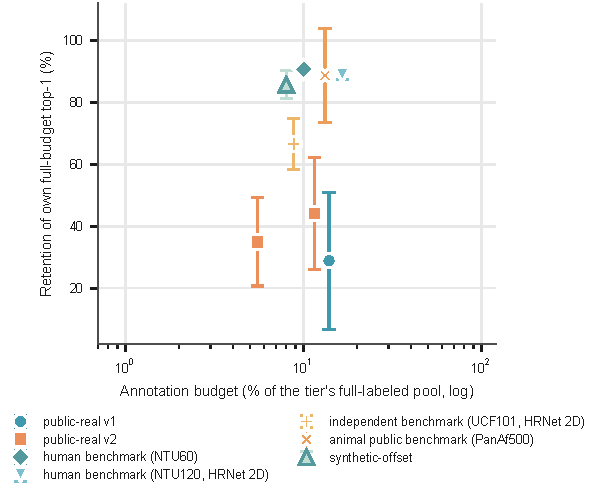
\includegraphics[width=0.76\linewidth]{fig5_budget_retention.pdf}
  \caption{Budget--retention summary: each point plots one tier's PSD pipeline at a labeled-data fraction against its retained full-budget top-1 (error bars: seed std; corrected protocol; the NTU60 error bar, $\pm$ 0.3\,pp, is smaller than its marker). The shaded 85--90\% band is the pre-registered PARTIAL decision band. Tier groups are never connected or pooled; near-coincident budgets are displaced along the log axis (v1 12.8\% shown at 13.9\%, v2 spc4 10.9\% at 11.5\%, synthetic-offset 9.1\% at 8.0\%, UCF101 10\% at 8.8\%, PanAf500 10\% at 13.2\%, NTU120 10\% at 16.5\%); plotted values, error bars, and ordinal axis spacing are unaffected. Retention is high on the human benchmarks under the interim supervised encoder (NTU60 90.7\%; NTU120 88.9\%, plotted; label-free pretext 74.96\%, FAILS, not plotted), on PanAf500 (88.7\% (plotted) at ten seeds; 85.8\% at thirty, interim encoder; 82.5\% label-free, FAILS, not plotted), and on the synthetic-offset tier, but collapses toward chance on the canine public-real tier at 13\%/5.5\% budgets (E7/E7b) and drops to 66.6\% on UCF101 (full-budget reference 23.1\%), bounded by pseudo-label quality, not budget arithmetic.}\label{fig:budget}
\end{figure}

\subsection{Comparison studies}\label{sec:comparison}

\emph{Tag disambiguation:} the reinforcement protocols reuse the tags E1--E3b with an explicit \emph{reinforcement} qualifier: Reinforcement E1 (same-episode zero-retraining bound), Reinforcement E2 (matched-budget three-arm contrast), and Reinforcement E3/E3b (split/addition episode and its labeled-budget ladder). These are distinct from the pipeline-stage experiments E1--E3 of Section~\ref{sec:main-results} (physics-layer representation quality, unsupervised segmentation quality, anchor-guided label expansion).

\paragraph{Implementation-equivalence verification on NTU60.}
Because AimCLR, SMQ, and the self-training machinery are re-implemented in this repository rather than imported, we verify implementation correctness on the human-domain benchmark (NTU RGB+D 60~\citep{shahroudy2016ntu}) before applying the pipeline to animal data. Following the linear-evaluation protocol of AimCLR~\citep{guo2022aimclr} on NTU60 cross-subject, each stream (joint, bone, motion) is pretrained for 300 epochs and evaluated with a frozen encoder and a fully-connected classifier, then fused with the official fixed weights (joint 0.6, bone 0.6, motion 0.4). The re-implementation reaches 74.30\% (joint), 71.51\% (bone), and 67.84\% (motion) top-1, and the three-stream fusion attains \textbf{77.97\% top-1 (95.78\% top-5; $n=16{,}487$)}, exceeding our pre-registered acceptance line of 77.18\% and lying within 0.93\,pp of the 78.9\% reported in the AimCLR paper body. We therefore treat the adapted implementation as equivalent to the official one for the purposes of this study. Throughout, baselines run under shared protocols; the head-to-head comparison below (Table~\ref{tab:h2h}) evaluates re-implemented published methods under an identical budget protocol, while no comparison against published \emph{reported} numbers is claimed (Section~\ref{sec:conclusion}, L13).

\paragraph{E9: low-resource retention on the human benchmark (C6, pre-registered).}
The animal-domain low-resource claim would be weak evidence if it did not generalize, so we pre-registered (PSD-NTU-PREREG-001, frozen before the experiment) a budget-shrinkage test on NTU RGB+D 60 cross-subject~\citep{shahroudy2016ntu}. Holding the frozen epoch-300 joint pretext backbone fixed, a 10\% class-stratified subset of the 40{,}091 training clips in the provider's frame-50 export yields 66.05\% with a linear head alone. Applying the PSD semantic pipeline (anchor-guided clustering with iterated confidence-filtered pseudo-labeling) under the corrected protocol of E7 yields \textbf{67.53\% $\pm$ 0.24} (ten seeds, after a 3-seed initial readout was expanded per the E9-series convention; both readouts released), which is \textbf{90.7\%} of the full-budget linear-probe reference of 74.45\% and clears the pre-registered generalization line of 90\%. The denominator is arm (c)'s linear probe, fixed at protocol freeze; under the three-stream fusion caliber of Section~\ref{sec:comparison} the same arms read 86.6\%. The linear-only arm alone already retains 88.7\% of the reference, so the pipeline's margin is modest: the pseudo-label iteration contributes $+1.48$\,pp over the linear-only arm (every seed arm above it; one-sample $t$ raw $p<10^{-7}$, Holm-corrected $p<10^{-6}$; Wilcoxon raw $p=0.002$, corrected $p=0.012$, under the series-wide eight-test family of Section~\ref{sec:implementation}). The labeled subset is $28\times$ larger than the animal-tier training pool (4{,}009 vs.\ 141 clips). An external semi-supervised baseline (PSD-SSL-BASE-001, frozen before the run) bounds this margin from below in the same harness (same frozen features, same 10\% subset, same evaluation): a Mean-Teacher-style~\citep{tarvainen2017mean} pool-distillation arm (soft pseudo-labels, $\tau{=}0.95$ confidence mask, five teacher--student rounds, ten seeds) reaches \textbf{46.79\% $\pm$ 0.61}, so the PSD pipeline exceeds it by $+20.7$\,pp (10/10 paired seed wins, Wilcoxon raw $p=0.002$, Holm-corrected $p=0.012$), while the baseline's confidence mask admits only 15{,}758 of 36{,}082 pool clips; near-full pool restoration is exactly what the confidence-thresholded baseline cannot do. On the weak-reference domain (UCF101) the same baseline lands at parity with its teacher (14.17\% vs.\ 14.04\%; PSD $+1.2$\,pp, n.s.), so the external-baseline disadvantage tracks the reference-quality gradient. Retention ratios are protocol-dependent (a frozen-probe budget-accuracy curve is flatter by construction than a fine-tuned pipeline's), so this arm supports the pipeline's own budget behavior and is not a comparison against any published method.

Four disclosures bound the reading: the pool adds $\approx$35.4k pseudo-labeled clips per seed (the near-restored training-set size \emph{is} the mechanism), and the gate accepts $\approx$98\% of the pool (the consensus gate is inert on the numeric NTU taxonomy), so this arm cannot separate filter quality from pool-size restoration (Section~\ref{sec:conclusion}, L11); the stopping rule is disabled on this tier, and pool precision against the official labels ($\approx$0.69) is a post-hoc diagnostic only; the 10\% subset is a single stratified draw (seed 42), so the $\pm$ 0.24 spread covers self-training seeds but not subset resampling; a post-hoc diagnostic redrawing the subset under four alternative seeds places the linear arm's spread at 65.62\% $\pm$ 0.48 (original 66.05\%, within one resample std; the decoupled arm's subset sensitivity is not measured); and the final head uses StandardScaler + logistic regression (tol $10^{-3}$) with the self-training head on GPU (scale adaptations, otherwise identical to E7).

\paragraph{Head-to-head against published methods under the identical budget protocol.}
The retention study above measures PSD against internal references; to situate the same arms against published methods, two published-method baselines are run in the identical harness on NTU60 cross-subject (Table~\ref{tab:h2h}): the AimCLR linear-evaluation arm (joint stream, official linear-probe recipe; the re-implementation verified above, with in-house pretext weights trained by the official recipe because the official released checkpoint was unreachable) and a supervised ST-GCN trained end-to-end on labels (reduced capacity: 16 hidden channels, 0.84M parameters; a deliberate small-capacity configuration for the 8\,GB GPU, so its accuracy is a same-harness supervised reference, not a reproduction of the published full-capacity model). Every arm consumes the same class-stratified subsets (per-class $k{=}\max(1,\mathrm{round}(f\,n_c))$; the 10\% arms on the protocol-frozen seed-42 draw of E9, 4{,}009 clips) or the full 40{,}091-clip training set, and is evaluated on the same 16{,}487-clip validation split; the PSD arms reuse the E9 numbers unchanged. Two lines of evidence support the 10\% ordering. On the protocol-frozen seed-42 draw, the PSD semantic pipeline reaches \textbf{67.53\% $\pm$ 0.24} (ten self-training seeds), above the AimCLR linear arm (\textbf{66.74\% $\pm$ 0.05} over five initialization seeds; $+0.79$\,pp, Welch $t{=}10.1$, raw $p{=}1.1\times10^{-6}$, Holm over the two post-hoc tests of this comparison $p{=}2.3\times10^{-6}$) and the end-to-end supervised arm (\textbf{64.84\% $\pm$ 2.18} over five initialization seeds; $+2.69$\,pp, Welch $p{=}0.051$, not significant, because one of the five initializations diverges to 61.30\% and inflates the arm's variance; the distribution-free Mann--Whitney test is significant at raw $p{=}6.7\times10^{-4}$, Holm-corrected $p{=}1.3\times10^{-3}$), with both published-method baselines landing within 1.3\,pp of the PSD linear head (66.05\%). On two independent stratified redraws of the 10\% subset (seeds 43/44, post-hoc; a single draw cannot separate draw quality from method effect), the ordering PSD $>$ AimCLR $>$ ST-GCN likewise holds on every draw, with PSD margins of $+7.8$/$+7.3$\,pp over AimCLR and $+10.0$/$+9.3$\,pp over ST-GCN. The pipeline itself is draw-sensitive (67.53\% on the frozen draw versus 74.11\% $\pm$ 0.22 and 74.20\% $\pm$ 0.08 on the redraws, with similar pool-restoration fractions, 97.9--98.7\% versus 95.2--96.1\%, so the gap reflects admitted pseudo-label quality rather than pool volume; the mechanism is not resolved and the per-draw diagnostics are released). A post-hoc budget extension on the same seed-42 draw (5\%/20\% columns of Table~\ref{tab:h2h}) shows the pipeline's advantage growing as the budget shrinks: at 5\% labels PSD reaches 74.20\% $\pm$ 0.05 versus 64.12\% (AimCLR linear) and 52.88\% (end-to-end ST-GCN), margins of $+10.1$/$+21.3$\,pp on the identical draw; and at 20\% 74.08\% $\pm$ 0.15 versus 69.62\%/72.83\%. The 10\% cell of the frozen draw sits below the pipeline's own 5\% and 20\% cells; we report this non-monotonicity as observed and do not fit a narrative to it. At full budget the ordering inverts: end-to-end supervised ST-GCN, consuming all 40{,}091 labels, dominates (83.46\%), while the frozen-feature arms cluster at 74.30\%/74.45\% (AimCLR linear / PSD linear probe). Job wall-clock on the same GPU: 2{,}268\,s (AimCLR) and 4{,}444\,s (supervised ST-GCN) for the original two-budget runs, plus a 20-cell robustness matrix (five-seed initialization block, two subset redraws, two budget extensions) of ${\sim}4.5$\,h total. Figure~\ref{fig:h2hbudget} plots the three budget points of Table~\ref{tab:h2h}. The same harness extends to the second benchmark: on NTU120 (E9b 12,000-clip/60-class subset, label-free physics layer), the linear head on the label-free features reads 44.18\% (the AimCLR linear-evaluation arm), the PSD semantic pipeline 43.75\% $\pm$ 1.16 (ten seeds; the $-0.43$\,pp margin of E9b), and end-to-end ST-GCN 36.17\% $\pm$ 1.71 (five initialization seeds): at this budget the frozen-feature arms sit ${\approx}8$\,pp above end-to-end training, reproducing the same-budget E2 pattern on a second benchmark, while the PSD-vs-AimCLR margin vanishes exactly as the label-free saturation analysis of E9b predicts.

\begin{table}[pos=htbp]
\centering
\caption{Head-to-head comparison on NTU60 cross-subject under an identical budget protocol: every arm trains on class-stratified labeled subsets of the same 40,091-clip training pool (per-class $k{=}\max(1,\mathrm{round}(f\,n_c))$; the 10\% arms use the protocol-frozen seed-42 draw of E9, 4{,}009 clips) and is evaluated on the same 16,487-clip validation split. Both published-method baselines are run by us: AimCLR linear evaluation (joint stream; re-implementation verified in the equivalence check, in-house pretext weights) and a reduced-capacity (16 hidden channels, 0.84M parameters) end-to-end supervised ST-GCN, a same-harness reference, not a reproduction of the published full-capacity model. The full-budget PSD reference is the frozen-feature linear probe; the semantic pipeline is not run at full budget. Baseline 10\% cells are means $\pm$ sample std over five initialization seeds (seed-0 runs included); the PSD 10\% cell reuses the E9 ten-self-training-seed readout; the 5\% and 20\% columns are a post-hoc extension on the same seed-42 draw (baselines: seed 0; PSD: three self-training seeds). At 10\% the PSD--AimCLR gap is $+0.79$\,pp (Welch $t{=}10.1$, raw $p{=}1.1\times10^{-6}$, Holm $p{=}2.3\times10^{-6}$) and PSD--ST-GCN is $+2.69$\,pp (Welch $p{=}0.051$, not significant; one divergent initialization at 61.3\%; Mann--Whitney raw $p{=}6.7\times10^{-4}$, Holm $p{=}1.3\times10^{-3}$). Subset-robustness redraws of the 10\% budget (seeds 43/44, post-hoc) preserve the ordering, with PSD margins of $+7.3$ to $+7.8$\,pp over AimCLR. The NTU120 block extends the same harness to the second benchmark under the label-free physics layer (E9b caliber; 10\% protocol-frozen draw); there the linear head on the label-free features already saturates the separable signal (44.18\%), and frozen features beat end-to-end training by ${\approx}8$\,pp (36.17\%).}
\label{tab:h2h}
\footnotesize
\hyphenpenalty=10000
\begin{tabularx}{\linewidth}{>{\raggedright\arraybackslash}X>{\raggedright\arraybackslash}p{1.7cm}>{\raggedright\arraybackslash}p{2.0cm}>{\raggedright\arraybackslash}p{1.7cm}>{\raggedright\arraybackslash}p{1.7cm}}
\hline
Method (NTU60 xsub; final block = NTU120) & 5\% labels & 10\% labels & 20\% labels & Full budget \\
\hline
Supervised ST-GCN, end-to-end (16 hid.\ ch., reduced capacity) & 52.88\% & 64.84\% $\pm$ 2.18 & 72.83\% & 83.46\% \\
AimCLR linear evaluation (joint stream, re-impl.) & 64.12\% & 66.74\% $\pm$ 0.05 & 69.62\% & 74.30\% \\
PSD linear head on frozen features (E9) & 63.30\% & 66.05\% & 68.79\% & 74.45\% \\
PSD semantic pipeline (E9 protocol) & 74.20\% $\pm$ 0.05 & 67.53\% $\pm$ 0.24 & 74.08\% $\pm$ 0.15 & -- \\
\hline
\multicolumn{5}{l}{\emph{NTU120 (E9b 12{,}000-clip/60-class subset; label-free physics layer; 10\% protocol-frozen draw; same harness)}} \\
Supervised ST-GCN, end-to-end (16 hid.\ ch., reduced capacity; 5 init.\ seeds) & -- & 36.17\% $\pm$ 1.71 & -- & -- \\
Linear head on the label-free features (= AimCLR linear evaluation; E9b) & -- & 44.18\% & -- & -- \\
PSD semantic pipeline (E9b protocol; 10 seeds) & -- & 43.75\% $\pm$ 1.16 & -- & -- \\
\hline
\end{tabularx}
\end{table}

\begin{figure}[pos=htbp]
  \centering
  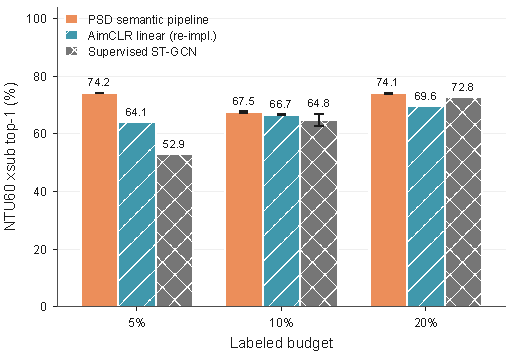
\includegraphics[width=0.76\linewidth]{fig7_h2h_budget.pdf}
  \caption{Head-to-head budget curve on NTU60 xsub (the harness of Table~\ref{tab:h2h}): top-1 of the PSD semantic pipeline, the AimCLR linear arm, and the end-to-end supervised ST-GCN at 5\%, 10\%, and 20\% class-stratified labeled budgets (bar means; error bars only where the released arm carries seed dispersion). The 10\% cells sit on the protocol-frozen seed-42 draw of E9; the 5\% and 20\% cells are the post-hoc extension on the same draw. Read the ordering across budgets from the figure; exact values, dispersions, and significance tests are in Table~\ref{tab:h2h} and the accompanying text.}\label{fig:h2hbudget}
\end{figure}

\paragraph{E9b/E9c: cross-domain retention gradient (pre-registered).}
To test whether the retention behavior is a property of the pipeline rather than of one benchmark, we pre-registered two further replications (PSD-NTU120-PREREG-001 and PSD-UCF101-PREREG-001, frozen before any run). On NTU RGB+D 120~\citep{liu2020ntu}, the official 3D-skeleton application was denied, so the replication uses the PYSKL-release HRNet 2D joint annotations (same video source and official labels, different extractor). It consumes a 12{,}000-clip, 60-class subset of the PYSKL NTU120 export, a caliber held identical across all arms (per-tier calibers in the supplementary material). The pretext is a joint-level MLP over all joint coordinates (80 epochs, frozen 256-d penultimate); this is a disclosed deviation from the frozen ST-GCN plan, adopted so one pretext architecture runs unchanged across both 17-joint benchmarks, with backbone quality absorbed by the full-budget reference arm. A supervision disclosure added in this revision: the interim MLP was trained with cross-entropy on the \emph{full} training labels, so on these tiers the frozen encoder is supervised, unlike the label-free contrastive physics layer used on NTU60 and claimed by the framework. At a 10\% stratified budget (ten seeds, after a 3-seed initial readout was expanded per the E9-series convention, adopted 2026-09-07 as a dated amendment; both readouts released; spreads cover self-training seeds but not subset resampling), the pipeline reaches \textbf{48.3\% $\pm$ 0.8} top-1 against the 10\%-linear arm's 45.4\% ($+2.9$\,pp; every seed arm above the linear arm). Significance tests use one-sample $t$ ($t{=}12.0$, raw $p<10^{-5}$) and Wilcoxon (raw $p=0.002$), Holm-corrected over the series-wide eight-test family (Section~\ref{sec:implementation}): corrected $p<10^{-5}$ and $0.012$, and conclusions are invariant to any narrower family choice. Retention against the full-budget reference's 54.3\% is \textbf{88.9\%, in the pre-registered PARTIAL band (85--90\%)}. A protocol-return amendment (2026-11-17) then executed the pre-registered physics layer itself on the identical 12{,}000-clip caliber: a from-scratch \emph{label-free} AimCLR pretext (ST-GCN base, 150 epochs, single joint stream, exactly as frozen in PSD-NTU120-PREREG-001; the 17-joint HRNet topology mapped into a fixed 16-active-slot arrangement on the 25-node NTU graph, nine dead slots, slot table in the supplementary material). Its full-budget reference (58.37\%) exceeds the interim encoder's (54.34\%), but the semantic pipeline reads 43.75\% $\pm$ 1.16 (ten seeds 42--51, completed in two sessions after a host-resource interruption; both logs released) against a 44.18\% linear head, a $-0.43$\,pp margin, for \textbf{74.96\% retention, FAILS}. Under the label-free pretext the linear head already saturates the separable signal at this budget, and pseudo-labeling adds nothing. Both readouts are released; neither supersedes the other (the interim verdict is the record of the executed-deviation protocol, the protocol-return is the record of the pre-registered one). On UCF101~\citep{soomro2012ucf101}, an independent third domain (YouTube-sourced video, 101 classes, HRNet 2D skeletons~\citep{sun2019hrnet}), the replication consumes a 10{,}000-clip subset under the same caliber (identical across arms; the official split-1 validation fold comprises 463 clips, part of the reported caliber). The same protocol yields \textbf{15.4\% $\pm$ 1.9} against a 14.0\% linear arm ($+1.4$\,pp; 8/10 seed arms above) and a 23.1\% reference; both tests are direction-consistent but neither significant (raw $t$ $p=0.049$, Wilcoxon raw $p=0.053$, Holm-corrected $p=0.141$ for both): \textbf{66.6\% retention, below the 85\% line, reported as a negative boundary}. The label-free protocol-return (2026-11-18) executes the pre-registered pretext on the identical 10{,}000-clip caliber: full-budget reference 19.87\% (vs.\ the interim encoder's 23.11\%), 10\% linear head 9.94\%, semantic pipeline 10.15\% $\pm$ 2.04 (ten seeds 42--51), a $+0.2$\,pp margin, for \textbf{51.09\% retention, FAILS}; both readouts are released. The external SSL baseline (Amendment 1 of PSD-SSL-BASE-001) extends to this domain: the Mean-Teacher arm reaches \textbf{14.17\% $\pm$ 0.87}, parity with its own teacher, the linear head (14.04\%), so the PSD pipeline's advantage over it is $+1.2$\,pp (8/10 wins, Wilcoxon raw $p=0.047$, Holm-corrected $p=0.141$; not significant). Where the full-budget reference is weak, confidence-thresholded pool distillation adds nothing: the same pretext-learnability gradient, now observed on the external-baseline axis.

Read together, the cross-domain points form a monotone gradient within the E9 series (NTU60 under the label-free AimCLR pretext; NTU120 and UCF101 under the interim supervised encoder). Retention falls from 90.7\% on NTU60 to 88.9\% on NTU120 and 66.6\% on UCF101 as the full-budget reference quality falls from 74.45\% to 54.3\% and 23.1\% (all E9-protocol linear-probe references; the AimCLR official-protocol re-implementation of the NTU60 reference is 74.30\%, Section~\ref{sec:comparison}). This indicates that what the frozen pretext learned about class-separable structure, not the budget arithmetic, bounds how far pseudo-label self-training can be stretched. The protocol returns isolate the encoder factor within tier. On NTU120, swapping the interim supervised encoder for the pre-registered label-free pretext raises the full-budget reference (54.34\% $\to$ 58.37\%) yet lowers retention (88.9\% $\to$ 74.96\%): on the label-free features the 10\% linear head already saturates the separable signal (44.18\%), so the pseudo-label pipeline's margin vanishes ($-0.43$\,pp). On UCF101 the same swap lowers both (reference 23.11\% $\to$ 19.87\%; retention 66.6\% $\to$ 51.09\%). On PanAf500 the swap raises the reference (60.0\% $\to$ 64.0\%) yet lowers retention (85.8\% $\to$ 82.5\%), the pipeline falling $7.2$\,pp below its own 10\% linear head. Under the single pre-registered label-free layer the ordering is monotone across all four executed tiers: retention 90.7\% $\to$ 82.5\% $\to$ 74.96\% $\to$ 51.09\% tracks reference quality 74.45\% $\to$ 64.0\% $\to$ 58.37\% $\to$ 19.87\% (NTU60/PanAf500/NTU120/UCF101). Retention is therefore a property of the physics layer's feature geometry, not of reference quality alone. The gradient claim is accordingly conditioned: \emph{within a fixed physics layer}, retention is monotone in full-budget linear-probe reference quality, with the high band (85--90\%) holding where the reference is separable and collapse where it is not. Any tier whose reference is strongly separable ($\geq$70\%) yet retains $<85\%$ at a 10\% budget under a fixed layer would break it; the pre-registered working-dog pilot is designed to supply such a test. This is the same mechanism boundary diagnosed on the canine tier (E7; the alignment analysis of Section~\ref{sec:conclusion}, L9), now observed on three additional public benchmarks. The low-resource claim is therefore scoped to tiers whose pretext features support linear separability at full budget, and the retention line is not claimed as a domain-universal property.

\paragraph{E9d: first animal-domain public benchmark (PanAf500, pre-registered).}
The mechanism boundary above predicts that retention depends on what the pretext learned, not on taxonomy, so it should extend beyond the human domain wherever a public animal benchmark exists. PanAf500 (great-ape natural behavior, in-the-wild video, 500 clips with official splits and nine behavior classes) is the public animal benchmark we could identify, and we pre-registered its budget-shrinkage test (PSD-PANAF-PREREG-001, frozen before any run) \emph{after} the E9b/c gradient was observable but \emph{before} the PanAf run executed. Its full-budget reference (60.0\%) lies below the $\geq$70\% falsifier threshold of the gradient's strong form, so this run is a directional consistency check rather than a potential falsifier: the observed retention (88.7\% at the pre-registered ten seeds; 85.8\% at the thirty-seed amendment below; both in the PARTIAL band) is consistent with the high band predicted for separable references. Skeletons are model-extracted: a YOLO11x-pose model fine-tuned on the ape subset of AP-10K (17-keypoint topology mapped onto the 24-slot PanAf extraction layout with seven dead slots; 17 active of 24 (an extraction-layout count), distinct from the 16-active/nine-dead arrangement of the 25-node NTU export mapping in the E9b/E9c calibration above) infers keypoints on bbox-cropped frames (82.1\% mean frame detection, 0.59 mean confidence; extraction noise enters all arms equally). Pretext, arms, budget, and decision rule mirror E9b/E9c. At a 10\% stratified budget (ten seeds), the pipeline reaches \textbf{53.2\% $\pm$ 9.1} against the 10\%-linear arm's 52.0\% and the full-budget reference's 60.0\%, for \textbf{88.7\% retention, in the pre-registered PARTIAL band} (a 3-seed early readout of 93.3\% fell into the CONFIRMS band and is superseded by the 10-seed number under the frozen rule; both released). The test split (75 clips, held out of the decision rule) yields 56\% as a non-decision secondary number. Two disclosures bound the reading: the nine-class space is long-tailed (three classes have $\le$7 clips; five classes contribute a single seed clip at the 10\% budget), inflating seed variance; and behavior labels are frame-level annotations majority-voted to clip level, the same coarse granularity diagnosed on the canine tier. PanAf500 completes the cross-domain picture at four points spanning two kingdoms. Under the interim supervised encoder, retention stays in the high band wherever the full-budget reference is separable (NTU60 90.7\%, NTU120 88.9\%, PanAf500 85.8\% at thirty seeds) and collapses where it is not (UCF101 66.6\%, reference 23.1\%). Executing the pre-registered label-free pretext on NTU120, despite its \emph{higher} reference (58.37\%), drops retention to 75.0\% (FAILS; rounded from the 74.96\% readout above); on UCF101 it lowers both the reference (23.1\% $\to$ 19.9\%) and the retention (66.6\% $\to$ 51.1\%, the rounded 51.09\%). On PanAf500 (2026-11-18 protocol return on the identical caliber; the PSD24 quadruped layout mapped to the same 16-active-slot arrangement, slot table in the supplementary material), the same swap raises the reference (60.0\% $\to$ 64.0\%) yet drops retention to \textbf{82.5\%, FAILS} (pipeline 52.8\% $\pm$ 9.6, ten seeds 42--51, against a 60.0\% linear head; interim readout 85.8\%, PARTIAL). This isolates the encoder's feature geometry as the binding factor (Section~\ref{sec:comparison}); budget retention is a property of pretext learnability, not of species or domain. The PanAf pipeline-vs-linear gap is not carried by the evidence at any tested power: at ten seeds it reads $+1.2$\,pp with 5/10 seed wins. A post-hoc seed expansion to thirty seeds (Amendment 2 of PSD-PANAF-PREREG-001, frozen before the run; seeds 42--71, both readouts released) gives 51.5\% $\pm$ 8.6 against the same linear arm (13/30 wins, 3 ties, Wilcoxon $p=0.54$), retention 85.8\%, verdict unchanged. The gap is therefore reported as directional only, and even $n{=}30$ does not separate the arms on this long-tailed nine-class space; as on NTU60, PanAf's retention is carried predominantly by the frozen-feature linear head, and no pipeline advantage is claimed on this tier.


\paragraph{E6-real-2: backbone-scale replication with matched solvers (pre-registered).}
TRANS-001's coupled arm retrains in $\approx$35\,s, so its cost endpoint was arithmetically unpassable: the replication could not have confirmed the cost claim at that scale. A second pre-registered replication (PSD-NTU-TRANS-002, frozen before the run; same $\mathcal{Y}\to\mathcal{Y}'$ merge, 60$\to$49 classes) therefore scales the backbone to the full ST-GCN of the equivalence verification and adds a third arm that decouples the two confounds TRANS-001 carried: the matched-solver arm (M) retrains a linear head on the coupled arm's own penultimate features with the decoupled arm's solver, isolating representation quality from retraining cost. As in TRANS-001, this merge-type transition admits the zero-retraining upper bound of Section~\ref{ssec:boundary}; the control is reported in Table~\ref{tab:attribution-controls}, whose same-episode ($60\to49$) bound rows carry the executed E1 reinforcement measurement (inference-only: 68.04\% rename-oracle upper / 67.97\% argmax-vote lower at the 10\% labeled head budget, zero retraining; protocol in the supplementary material). Full budget (40,091 clips, seeds 42--44): the coupled arm retrains in a median of 9897\,s against the decoupled head's 626\,s (15.8$\times$; verdict \textbf{PARTIAL} per the frozen rule), accuracy 79.8\% (coupled) vs 75.3\% (decoupled, gap $-4.5$\,pp). A first run at the nominal scaled learning rate collapsed to a constant predictor mid-training on all three seeds (NaN) and was discarded under a NaN watchdog added to the protocol; the reported run uses half the linear-scaled learning rate. All three coupled-arm seeds include host-restart segments; wall-clock is the sum of contributing segments per seed, with the per-segment decomposition in the released artifact. The verdict is robust to the accounting: a final-segment-only bound (6.2$\times$) still clears the $3\times$ line. At the 10\% budget the same replication reads 32.5$\times$ (coupled 1520\,s vs decoupled 47\,s; ratio on unrounded seconds) with a $+2.6$\,pp decoupled advantage (\textbf{PARTIAL} at the 10\% tier). A dated addendum (PSD-NTU-TRANS-002-MEXP, frozen before the expansion ran) replicated the matched-solver comparison over ten seeds (42--51; the three seeds above reused unchanged): the matched-solver arm exceeds the coupled arm on every seed (mean 82.6\% vs 79.7\% over ten seeds; the three-seed frozen-budget comparison above reads 82.6\% vs 79.8\%; $+2.9$\,pp; paired Wilcoxon $p=0.002$, sign test 10/10; two-test addendum family, Holm-adjusted $p=0.004$). End-to-end training under-exploits its own representation, and the frozen cost-ratio verdict is unaffected. A CIL-flavored reference adapted to this episode (LwF-style distillation from the $\mathcal{Y}$-era head with merge-aggregated targets plus old-class replay; protocol and adaptation freedom in the supplementary material) lands between the bound and the coupled arm: \textbf{68.6\% $\pm$ 0.4} at the 10\% labeled head budget and \textbf{72.9\% $\pm$ 0.04} at the full budget (three seeds), comparable to the decoupled rebuild at 10\% (67.6\%) and below it at the full budget (75.3\%), so a CIL-style alternative does not dominate the decoupled structure where the retraining cost is actually saved.

\paragraph{Reinforcement E3: residual value on a split/addition transition (specified in advance, same-day).}
The merge replications above exercise transitions that a frozen $\mathcal{Y}$-era model can absorb without any new supervision; the complementary question is what decoupling is worth when the transition \emph{requires} new supervision. On the synthetic tier, a split/addition episode ($\mathcal{Y}\to\mathcal{Y}'$: $22\to29$ classes, where three parents each split into two children whose parent samples are unavailable in $\mathcal{Y}'$, plus four brand-new classes with no $\mathcal{Y}$-era source; protocol in the supplementary material) probes the new-supervision ladder with four arms (seeds 42--44): the zero-shot remap of the frozen $\mathcal{Y}$-era head cannot name any new class (0\% on the additions; 43.0\% overall), the decoupled semantic rebuild with $k{=}10$ new labels per new class reaches 45.7\% overall (E3's own 50-clip/class pool; the E3b ladder enlarges the pool to 100 clips/class and reads 45.3\% $\pm$ 0.2 at the same nominal $k{=}10$, Table~\ref{tab:kladder}), a frozen head trained on the full $\mathcal{Y}'$ labeling reaches 68.0\%, and coupled full retraining reaches 97.1\%. The decoupled rebuild spends $5\times$ fewer new labels than the coupled arm (100 vs.\ 500) at $3.02\times$ lower median wall-clock (50.6\,s vs.\ 153.0\,s); under the E6 decision rule the episode returns \textbf{PARTIAL}: the cost line is cleared, but the $-51.4$\,pp accuracy gap exits the $\pm2.3$\,pp band. Whether that gap closes as the decoupled arm's label budget grows is the subject of the ladder below.

\paragraph{Reinforcement E3b: labeled-budget ladder on the split/addition episode ($k\in\{10,25,50,100\}$; specified in advance, same-day).}
The ladder holds the E3 episode fixed and grants the decoupled arm exactly $k$ stratified fresh labels per new class (the 19 retained classes keep their $\mathcal{Y}$-era labels via remap), while the coupled and frozen-head arms consume the full $\mathcal{Y}'$ labeling as $k$-independent references (Table~\ref{tab:kladder}; protocol in the supplementary material). Two caliber disclosures: the annotation pool is enlarged from 50 to 100 clips per class so the $k{=}100$ rung is drawable, making $k{=}10$ a trend reference rather than an exact replication of E3; and the coupled and frozen-head arms are $k$-independent, so their three-seed readout is reused at every rung. Every rung is reported as the mean $\pm$ s.d.\ over seeds 42--44; seeds 43--44 at $k\in\{10,25,50\}$ were added by a same-day supplemental run, and the initial single-seed and merged three-seed readouts are both released. The decoupled arm rises monotonically from 45.3\% to 72.4\% but saturates at the frozen-feature ceiling: at $k{=}100$ it coincides with the frozen-head arm (72.4\% vs.\ 71.7\%; same frozen path, same full new-label budget), while the coupled arm holds at 95.9\%$\pm$0.5. The margin never leaves 23.45--50.57\,pp, far outside the $\pm2.3$\,pp parity band, so no critical $k^{\ast}$ exists within the tested range: the residual-value hypothesis is \emph{not supported at any tested budget}. Decoupling's measured value here is confined to label and wall-clock savings (at $k{=}10$: 100 vs.\ 1{,}000 new labels; 92\,s vs.\ 234\,s, seed 42); closing the accuracy gap appears to require adapting the frozen encoder rather than adding labels. Figure~\ref{fig:kladder} plots this ladder readout against the two $k$-independent references and the $\pm2.3$\,pp parity band.

\begin{table}[pos=htbp]
\centering
\caption{Labeled-budget ladder on the synthetic split/addition episode (reinforcement E3b; $22\to29$ classes; episode fixed at seed 42; every cell is the mean $\pm$ s.d.\ over seeds 42--44; the coupled and frozen-head arms consume the full $\mathcal{Y}'$ labeling and are therefore $k$-independent references, identical across rungs). The annotation pool is 100 clips per class, so the $k{=}10$ rung is a trend reference rather than an exact replication of E3. The coupled-minus-decoupled margin stays far outside the $\pm2.3$\,pp parity band at every rung: no critical $k^{\ast}$ exists within the tested range.}
\label{tab:kladder}
\footnotesize
\hyphenpenalty=10000
\begin{tabularx}{\linewidth}{>{\raggedright\arraybackslash}p{2.2cm}>{\raggedright\arraybackslash}p{2.2cm}>{\raggedright\arraybackslash}p{2.0cm}>{\raggedright\arraybackslash}p{2.0cm}>{\raggedright\arraybackslash}X}
\hline
New labels per class $k$ (total) & Decoupled rebuild top-1 & Coupled top-1 ($k$-indep.) & Frozen head top-1 ($k$-indep.) & Coupled $-$ decoupled margin \\
\hline
10 (100) & 45.3\% $\pm$ 0.2 & 95.9\% $\pm$ 0.5 & 71.7\% $\pm$ 0.5 & 50.57\,pp \\
25 (250) & 59.1\% $\pm$ 2.5 & 95.9\% $\pm$ 0.5 & 71.7\% $\pm$ 0.5 & 36.78\,pp \\
50 (500) & 65.1\% $\pm$ 1.3 & 95.9\% $\pm$ 0.5 & 71.7\% $\pm$ 0.5 & 30.80\,pp \\
100 (1{,}000) & 72.4\% $\pm$ 0.0 & 95.9\% $\pm$ 0.5 & 71.7\% $\pm$ 0.5 & 23.45\,pp \\
\hline
\end{tabularx}
\end{table}

\begin{figure}[pos=htbp]
  \centering
  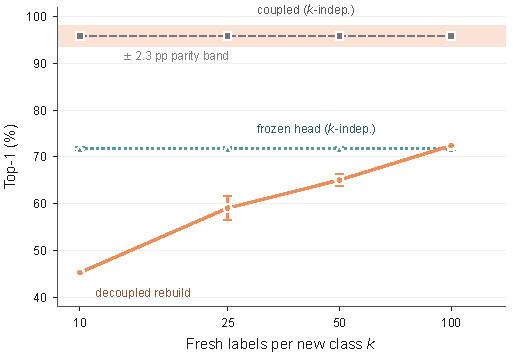
\includegraphics[width=0.76\linewidth]{fig6_kladder.pdf}
  \caption{Labeled-budget ladder on the synthetic split/addition episode (reinforcement E3b; readout of Table~\ref{tab:kladder}): top-1 of the decoupled semantic rebuild as its fresh-label budget $k$ per new class grows (seeds 42--44; error bars: seed s.d.). The coupled and frozen-head arms consume the full $\mathcal{Y}'$ labeling and are drawn as $k$-independent horizontal references; the shaded band is the $\pm2.3$\,pp parity band around the coupled arm. The decoupled arm rises monotonically yet saturates at the frozen-feature ceiling, and its margin to the coupled arm never enters the band; exact per-rung values are in Table~\ref{tab:kladder}.}\label{fig:kladder}
\end{figure}

\paragraph{Segmentation strategy.}
Under the seeds pseudo-ground-truth protocol (Section~\ref{sec:ablation}), motion-word quantization (0.458$\pm$ 0.049) leads the equal-segment-count uniform-window arm (0.399$\pm$ 0.035) and the random-cut null (0.323$\pm$ 0.022), passing all three pre-registered gates; a fixed-grid probe (0.453$\pm$ 0.027) is statistically on par, and uniform windows lead on boundary F1 (0.396 vs.\ 0.343). Per the downgraded positioning of SMQ (an auxiliary proposal source), no end-to-end recognition advantage is claimed from these numbers alone; the dedicated downstream ablation (equal-count fixed windows under the identical frozen-feature head) attributes $\Delta = 0.0$ clip-level accuracy to SMQ (Section~\ref{sec:ablation}), and the full end-to-end pipeline attribution remains future work.

\paragraph{End-to-end comparison against training from scratch.}
A five-arm study on the same 12-class protocol (three seeds; full protocol and per-arm numbers in the supplementary material) completes the matrix: under the frozen-head protocol (the usage mode our decoupled design prescribes), the pretrained backbone outperforms a random one by $+8.3$\,pp (35.71\% vs.\ 27.38\%), whereas under \emph{full} fine-tuning the advantage disappears (36.90\% vs.\ 36.90\%; the scratch arm attains the best macro-F1), corroborating the gradient-ablation crossover of Section~\ref{sec:ablation}: past the crossover budget the pretrained prior adds no value \emph{as a fine-tuning initialization}. Every deep arm and a flatten-plus-logistic baseline cluster in a narrow 27--37\% band (random 6.0\%, majority 25.0\%): the tier's ceiling is set by the self-extraction data bottleneck, not by the choice of model. Reference calibers on this tier (33.93/35.71/36.90/37.50/35.42\%) span up to 3.6\,pp, a caliber effect, not a model effect; within-protocol arm comparisons are unaffected.

\paragraph{Scope statements.}
The NTU60 equivalence verification covers the AimCLR pretraining and three-stream fusion protocol; SMQ is validated through pre-registered ablation comparisons rather than against an official baseline protocol (none is published), and the TCL-style self-training is delivered as an equivalent iteration loop since no official implementation exists (Section~\ref{ssec:selftrain}). Two further registered comparisons remain outside the present evaluation and are not claimed anywhere in this paper: the AimCLR++ backbone variant (80.9\% NTU cross-subject per the official repository's linear-evaluation table) as an alternative physics-layer encoder, and exhaustive sweeps over the confidence threshold $\tau$ and cluster count $K$.

\begin{table}[pos=htbp]
\centering
\caption{Main results under the three-tier protocol (plus the public human-domain benchmark used for implementation-equivalence verification). Tiers are never mixed; the real-K9 row is blank because that tier is not exercised (Section~\ref{sec:datasets}); per-class breakdowns accompany the four-class public-real aggregate (Section~\ref{sec:conclusion}); attribution controls are consolidated separately in Table~\ref{tab:attribution-controls}. The synthetic full-budget reference (96.6\%) is a single seed-42 run without dispersion; retention figures using it as denominator inherit that caliber.}
\label{tab:main}
\footnotesize
\hyphenpenalty=10000
\begin{tabularx}{\linewidth}{>{\raggedright\arraybackslash}p{2.7cm}>{\raggedright\arraybackslash}X>{\raggedright\arraybackslash}p{1.2cm}>{\raggedright\arraybackslash}p{4.1cm}}
\hline
Tier & Task / protocol & Metric & Result \\
\hline
Synthetic & 22-class, full budget (matched 50-ep) & top-1 & 96.6\% (single run, seed 42) \\
Synthetic-offset & 22-class, 20-clip warm-start & top-1 & 82.0\% ($\pm$ 4.3) \\
Synthetic & taxonomy transition, decoupled vs.\ full & wall-clock & 31.1\,s vs.\ 188.7\,s ($6.07\times$; $\geq 3\times$ claimed) \\
\hline
Public-real & $k$-NN subject probe (representation) & top-1 & 20.89\% ($2.51\times$ random) \\
Public-real & segmentation IoU (seeds pseudo-GT) & IoU & 0.458 $\pm$ 0.049 \\
Public-real & prototype purity (InterPet4D 7-label seed space) & purity & 0.5339 ($1.61\times$ random; $+4.8$\,pp majority) \\
Public-real & pseudo-label pool precision (round-1 endpoint) & prec. & 0.691 $\pm$ 0.013 (paired first-to-last n.s.) \\
Public-real & 4-class partial, frozen backbone + head & top-1 & 41.5\,$\pm$\,5.9 (3 seeds; best 44.90\%; per-class in Section~\ref{sec:conclusion}, L7) \\
Public-real & 12-class two-arm (warm vs.\ random backbone) & top-1 & 35.71\% vs.\ 27.38\% \\
Public-real & 12-class two-arm under full fine-tuning (null; five-arm study) & top-1 & 36.90\% vs.\ 36.90\% \\
Public-real & end-to-end PSD pipeline @ 13\% budget, corrected pseudo-label protocol (10 seeds) & top-1 & 9.8\% (chance 11.1\%; negative boundary, E7) \\
Public-real & generic-SSL control @ 13\% budget (10 seeds) & top-1 & 15.2\% $\pm$ 5.1 (above pipeline; E7) \\
Public-real (v2 replication) & same corrected protocol, expanded tier @ 2 clips/class (10 seeds) & top-1 & 13.1\% (chance 12.5\%; E7b) \\
\hline
Public human benchmark & NTU60 xsub 3-stream fusion (equivalence) & top-1 & 77.97\% (line: 77.18\%) \\
Public human benchmark & PSD pipeline @ 10\% labels, corrected protocol (E9, retention) & top-1 & 67.5\% (90.7\% of linear-probe ref 74.45\%; line: 90\%, ten seeds) \\
Public human benchmark (HRNet 2D) & NTU120 replication @ 10\% labels, corrected protocol (E9b, retention) & top-1 & 48.3\% interim supervised encoder (88.9\% of probe ref 54.3\%; PARTIAL band 85--90\%, ten seeds); 43.75\% pre-registered label-free pretext (74.96\%, FAILS; Section~\ref{sec:comparison}) \\
Animal public benchmark (PanAf500) & PSD pipeline @ 10\% labels, corrected protocol (E9d, retention) & top-1 & 51.5\% interim supervised encoder (85.8\% of probe ref 60.0\%, thirty seeds; ten-seed readout 53.2\%/88.7\%; PARTIAL band); 52.8\% pre-registered label-free pretext (82.5\%, FAILS; Section~\ref{sec:comparison}) \\
Independent benchmark (HRNet 2D, YouTube) & UCF101 @ 10\% labels, corrected protocol (E9c, retention) & top-1 & 15.4\% (66.6\% of probe ref 23.1\%; negative boundary, ten seeds) \\
\hline
Real-K9 & -- & -- & not exercised in this study \\
\hline
\end{tabularx}
\end{table}

           % hist-draft: experiment-skeleton.md §4 (三层口径铁律随行)
% 05-ablation-analysis.tex — truth: 本文件（2026-09-10 交割：R22 后全部正文修订直改 tex，原装配源 md 已冻结为历史设计稿，见其头部治理注记）
% 纪律: E5 探索性发现措辞按裁决①(效率主张禁用); tab3 表格 + 低资源梯度段(成对呈现纪律: 低资源档与饱和档必须成对出现);
% fig4 caption 逐字取 FIGURE_SOURCE.md; 四步分析结构 observe→interpret→implicate→next。
\section{Ablation and analysis}\label{sec:ablation}

Table~\ref{tab:ablation} summarizes the component-level ablations; each row removes, replaces, or perturbs one design element and reports the measured consequence under its disclosed caliber.

\begin{table}[pos=htbp]
\centering
\caption{Component ablations. Every number is tier-tagged; tiers are never mixed. Paired designs are described inline. Device calibers are disclosed where a row spans devices (row 1: gradient tiers CPU, saturation tier GPU); cross-device absolute accuracies are not poolable (Section~\ref{sec:conclusion}, L10).}
\label{tab:ablation}
\footnotesize
\hyphenpenalty=10000
\begin{tabularx}{\linewidth}{>{\raggedright\arraybackslash}p{2.6cm}>{\raggedright\arraybackslash}p{1.8cm}>{\raggedright\arraybackslash}X}
\hline
Switch & Claim & Result (caliber) \\
\hline
$-$ self-supervised pretraining & C3 & Benefit decays to statistical equivalence with budget: $+21.2$\,pp at 88 clips (scratch $\approx$2.3$\times$ random), $+9.9$\,pp at 176, $-2.3$\,pp at 352 (crossover), $+0.15$\,pp n.s.\ at 1760 \emph{(synthetic; scratch vs.\ warm, 3 seeds; gradient tiers CPU, saturation GPU)} \\
$-$ semantic warm-start (generic-SSL instead) & C6 & Corrected end-to-end protocol (final head on seed truth + pool pseudo-labels; 10 seeds at 2 and 4 clips/class; full-budget arm deterministic): both arms near chance at 2 clips/class (top-1 9.8 vs.\ 15.2; macro-F1 5.3 vs.\ 10.4, Holm-corrected $p=0.023$ favoring generic-SSL), same ordering at 4 (top-1 10.9 vs.\ 15.9, n.s.; macro-F1 7.3 vs.\ 13.9, corrected $p=0.049$); at full supervision the reference still favors the task-pretrained backbone (33.93 vs.\ 30.36). The earlier warm-start advantage at low budget was an artifact of a true-label head and is superseded \emph{(public-real; AimCLR@InterPet4D, mocap domain gap disclosed)} \\
$-$ unsupervised segmentation (replace SMQ) & C4 (auxiliary) & SMQ 0.458$\pm$ 0.049 $>$ uniform window 0.399$\pm$ 0.035 $>$ random-cut null 0.323$\pm$ 0.022; all three pre-registered IoU gates pass. A fixed-grid probe (0.453$\pm$ 0.027) is on par with SMQ, and uniform windows lead on boundary F1 (0.396 vs.\ 0.343)---no consistent SMQ advantage. SMQ is positioned as an auxiliary proposal source; a downstream ablation swapping SMQ's proposals for equal-count fixed windows under the same frozen-feature head measures identical clip-level accuracy (45.95\% vs.\ 45.95\%, $\Delta = 0.0$) \emph{(public-real; seeds pseudo-GT, 4 episodes)} \\
$-$ anchor guidance & C5 & Prototype purity drops from 0.5339 to a 0.3306 random-assignment baseline ($1.61\times$; all-majority baseline 0.4858); seed-ratio 25\%$\to$100\% adds $\leq$1\,pp at $K\in\{5,10\}$ but costs 2.4\,pp at the best sweep cell $K{=}14$ \emph{(public-real / P0.3)} \\
$-$ pseudo-label iteration (single round) & C5 & Pool precision 0.5125 $\to$ 0.6913 ($+17.9$\,pp at round 1, a point estimate); the pre-registered first-to-last comparison over all iterated rounds is direction-consistent but \textbf{not significant after Holm--Bonferroni correction} (corrected $p=0.090$ over the three-test family; raw $p=0.030$); the precision-drop stopping rule fired after two degraded rounds, selecting round~1. We claim \emph{no robust benefit from multiple iterations}: round-1 is the reported operating point, multi-round gains directional only, a dedicated multi-round ablation registered as future work \emph{(public-real / P0.4, physics-prior consensus caliber)} \\
$-$ uncertainty sampling (use random) & C7 (exploratory) & No entropy advantage under cold-start weak scorers: random leads in mean by $+7.9$\,pp at budget 100 (2/3 seeds) and $+7.1$\,pp at 200 (3/3 seeds); direction confirmed with strong in-domain scorers ($+4.2$--$5.0$\,pp at every budget above the shared initial set) \emph{(synthetic; negative result)} \\
seed-noise injection \{10/20/30\%\} & C5 & Purity 0.5339 $\to$ 0.5267 $\to$ 0.5201 $\to$ 0.5025 at 30\% ($-3.1$\,pp, still $1.52\times$ baseline)---iteration does not amplify seed noise at this scale \emph{(public-real / P0.3)} \\
\hline
\end{tabularx}
\end{table}

\paragraph{Pretraining value is a function of annotation scarcity.}
Across four matched budgets (88/176/352/1760 clips, scratch vs.\ pretraining-initialized, three seeds each), the fine-tuning benefit decays to statistical equivalence: $+21.2$\,pp at 88 clips (scratch $\approx$2.3$\times$ random, warm $7\times$), $+9.9$\,pp at 176 (warm-start std $3.8\times$ narrower), $-2.3$\,pp at 352 (crossover region, within one arm's std), $+0.15$\,pp (n.s.) at 1760. The zero crossing lies between 10 and 20 clips per class; the bracket is the claim, and low-resource and saturated tiers are reported paired throughout. Together with the $k$-NN probe of Section~\ref{sec:main-results} (E1), this gives two complementary lines of evidence for C3: representation discriminability (probe) and fine-tuning value (gradient). Mechanism: the scarcer the labels, the less a discriminative representation can be learned from data, and the cross-domain prior of the pretraining-initialized encoder becomes the dominant usable structure at the smallest budgets.

\paragraph{Segmentation component status (downgraded).}
SMQ's IoU advantage over the uniform-window arm (0.458 vs.\ 0.399) does not extend to boundary F1 (0.343 vs.\ 0.396), and the fixed-grid probe is on par (0.453 $\pm$ 0.027); evaluation uses seed-derived pseudo-ground truth over four episodes. A dedicated downstream recognition ablation isolates SMQ's contribution directly: on the public-real tier (7-class seed-pseudo-GT caliber, 151/74 train/val clips), replacing SMQ's proposals with equal-count fixed windows under the identical frozen-feature linear head yields identical clip-level accuracy (45.95\% vs.\ 45.95\%, $\Delta = 0.0$). SMQ is therefore treated throughout as an auxiliary proposal-generation step inherited from prior work~\citep{gokay2025smq}, not a validated contribution; the claims of Section~\ref{sec:main-results} do not rest on it.

\paragraph{Multi-round pseudo-label iteration: no robust benefit.}
The round-1 endpoint gain in pool precision ($0.5125 \to 0.691$, $+17.9$\,pp) is real but is a point estimate; the pre-registered paired first-to-last comparison over all iterated rounds yields $\Delta$ $+10.69 \pm 3.28$\,pp with raw $p=0.030$, \emph{not} significant after Holm--Bonferroni correction over the three-test family (corrected $p=0.090$). The precision-drop stopping rule fired after two consecutive degraded rounds, selecting round~1 as the reported operating point. We make no claim that multiple iterations improve the pipeline: all reported operating points use round~1, the first-to-last trend is direction-consistent only, and a controlled multi-round ablation is registered as future work.

\paragraph{Semantic warm-start versus generic-SSL on real skeletons.}
The synthetic-tier row above asks whether pretraining helps at all; on the public-real tier we ask the sharper question of \emph{which} pretraining earns the low-label budget. Holding the entire end-to-end pipeline fixed (seeds, anchor-guided pseudo-labeling, head, splits, leakage guards) and replacing the backbone initialization together with its bound native input preprocessing (each arm uses the preprocessing its method was trained with; disclosed)---task-pretrained semantic warm start versus a generic contrastive encoder pretrained on motion-capture dog skeletons (AimCLR)---the corrected pseudo-label protocol finds both arms at or near chance at 2 clips/class (top-1 9.8\% vs.\ 15.2\%; chance 11.1\%), with the generic-SSL arm ahead on macro-F1 (10.4\% vs.\ 5.3\%, per-tier Holm-corrected $p=0.023$) and the same ordering at 4 clips/class; at full supervision the deterministic supervised reference still favors the task-pretrained backbone (33.93\% vs.\ 30.36\%; Section~\ref{sec:main-results}, E7c). The generic arm carries a mocap-to-in-the-wild domain gap its original evaluation did not: it is a transfer lower bound, not a best-tuned AimCLR. The reading is a boundary condition rather than a mechanism: at a 13\% budget on this tier, neither initialization yields pseudo-labels good enough to train on, and the earlier warm-start advantage---obtained under a protocol that trained the final head on pool ground truth---does not survive the correction. What the tier's supervised comparisons support (E4 pool precision, direction-consistent but corrected $p=0.090$; the five-arm study in Section~\ref{sec:comparison}) is that task-pretrained features are better when labels are present. The released per-arm pool-precision diagnostics ($0.11$ warm vs.\ $0.15$ generic-SSL) suggest pseudo-label quality does \emph{not} track supervised feature quality at budget---a post-hoc observation, not a controlled test.

\paragraph{Canine rescue levers: three pre-registered nulls.}
The alignment, backbone-adaptation, and budget levers below were pre-registered to rescue the canine tier's low-budget failure (Section~\ref{sec:main-results}, E7). All three returned null, and we consolidate them here as the boundary-condition evidence referenced in Section~\ref{ssec:boundary}.

\paragraph{Label-alignment force: a pre-registered null on the canine tier.}
The E7/E7b negative boundary raises the question of whether a stronger pseudo-label correction can rescue the canine tier at a 13\% budget. We pre-registered (PSD-ALIGN-PREREG-001, frozen before the run) three ground-truth-free alignment mechanisms against the R16 control, all sharing the corrected protocol and differing only in how the seed-anchored prototype geometry constrains pseudo-labels: V1 requires head--prototype top-1 agreement for pool entry, V2 adds a seed-prior per-class quota, V3 lets the prototype path assign throughout. Over ten seeds on AK v1 spc2, the best variant (V2) reaches 14.1\% $\pm$ 6.7 top-1---winning 8 of 10 same-seed pairs against the control (9.8\%, mean $+4.3$\,pp, Wilcoxon raw $p=0.13$, not significant)---and V3 roughly doubles pool pseudo-label precision (0.21 vs.\ control 0.11)---but the pre-registered rescue bar (mean $\geq 20\%$) is not met, so the decision rule returns \textbf{NULL}. We report this as a bounded negative (the first of three null rescue levers, Section~\ref{ssec:boundary}): the alignment force improves pseudo-label quality and is directionally consistent, but on this tier the binding constraint is the seed-anchored feature geometry itself (r0 prototype precision $\approx$0.30 caps what any gate can select), not the gating rule---consistent with the label-in-the-loop diagnosis of Section~\ref{sec:conclusion} (L9). Evidence: the released experiment ledger.

\paragraph{Two further levers: backbone adaptation and label budget, both null.}
If gating was not the binding constraint, two orthogonal levers remain: a stronger backbone and more labels. We pre-registered both (PSD-DAP-PREREG-001, PSD-BUDGET-PREREG-001; ADR 0008). \emph{Backbone}: domain-adaptive continued pretraining (two-view InfoNCE) on 503 unlabeled APTv2 canid skeleton clips, initialized from the physics-layer backbone. A pre-registered fidelity self-check fired first---the full-supervision reference on AK dropped from 33.93\% to 25.0\% ($<$30\% line), i.e.\ catastrophic forgetting---and the adapted backbone did not help downstream (V2+DAP 11.4\% vs.\ 14.1\% for the P1 gate, paired wins 3/10), corroborating that APTv2$\to$AK is bottlenecked by topology/appearance mismatch rather than adaptation strength. \emph{Budget}: sweeping the seed budget from spc2 (13\% labels) to spc12 (77\% labels), the best variant (V2) rises only from 14.1\% to 22.1\% and never reaches the 24\% (70\%-retention) knee at any budget; the pseudo-label pool (precision 0.04--0.17) adds no measurable value over the seed-only arm. Three independent levers---gating, backbone, budget---thus agree: on the AK self-extraction tier the end-to-end low-resource claim is not rescued by any lever we tested, and the binding constraint is the tier's data quality itself; the three nulls jointly constitute the boundary condition analyzed in Section~\ref{ssec:boundary}. The pre-registered real-K9 pilot (Section~\ref{sec:datasets}) is designed to test this falsification on target-domain data of adequate quality. Evidence: the released experiment ledger.

\paragraph{Uncertainty sampling: an exploratory negative finding (C7, downgraded by pre-registration).}
As an exploratory finding, uncertainty sampling did not help in our regime. Under cold-start weak scorers on the synthetic tier, entropy sampling showed no detectable advantage: random led in mean by 7.9\,pp at budget 100 (2 of 3 seeds) and 7.1\,pp at 200 (3 of 3 seeds); a full-budget rerun reproduces the direction (12.3/7.8\,pp), and with warm-started in-domain scorers random still led by 4.2--5.0\,pp at every budget above the shared initial set ($b\geq 50$). A diagnostic explains the mechanism: the synthetic-trained checkpoint scored the public-real pool with fully saturated softmax (mean top1$-$top2 logit margin 100.9 vs.\ $\approx$10.8 in-domain), reducing uncertainty signals to numerical zero---the classical preconditions of uncertainty sampling (a strong scorer, in-domain calibration) are exactly what a low-resource pipeline lacks at startup. This motivates a progressive annotation narrative (annotate first, calibrate the scorer, then select), left to future work. Figure~2 of the supplementary material shows both protocols.

\paragraph{Sensitivity.}
Seed-ratio sweeps show prototype quality saturating early ($\leq$1\,pp beyond 25\% seeds at $K\in\{5,10\}$; $-2.4$\,pp at the best sweep cell $K{=}14$); the confidence threshold $\tau$ and cluster count $K$ interact with the frequency-aware margin design, and full sweeps are registered as future work. The class-imbalance handling switch (frequency-aware margins vs.\ resampling) is registered for evaluation on the public-real tier (not yet run) together with the per-class breakdown mandated by Section~\ref{sec:conclusion}.
     % hist-draft: experiment-skeleton.md §5 (tab3 七行零 PENDING)
% 06-conclusion-limitations.tex — truth: 本文件（2026-09-10 交割：R22 后全部正文修订直改 tex，原装配源 md 已冻结为历史设计稿，见其头部治理注记）
% 纪律: 结论段逐字搬运; Limitations 十二条独立成段 (L1-L12; 终审 2026-09-07 勘正条数); rebuttal 预案不入正文(投稿期备用)。
\section{Conclusion and limitations}\label{sec:conclusion}

\subsection{Conclusion}

We presented PSD, a physics--semantics decoupled framework for skeleton-based behavior recognition under evolving evaluation criteria: a label-free physics layer provides self-supervised dynamics representations and unsupervised behavior proposals, while a lightweight semantic layer grows rule-engine seeds toward full taxonomy coverage through anchor-guided clustering, single-round confidence-filtered pseudo-labeling, and warm-started small-budget initialization. Experiments across the two exercised tiers and four public benchmarks spanning two kingdoms (NTU60, NTU120, UCF101, PanAf500) showed that pretraining yields discriminable dynamics representations ($2.51\times$ random baseline; a subject-identification probe, not a behavior measure), that the semantic layer attains \textbf{82.0\% top-1 on 22 classes from a 20-clip budget via warm-started initialization} (synthetic-offset tier, vs.\ 96.6\% full-budget; the 20 clips are the marginal budget atop a fully labeled source domain; $\pm$ 4.3 across three seeds), and that synthetic-tier taxonomy transitions are absorbed at \textbf{$\geq 3\times$ lower wall-clock retraining cost} at matched accuracy (measured $6.07\times$; accuracy differences inside the pre-registered $<2.3$\,pp noise band), with real-domain replications returning FAIL at MLP scale and PARTIAL at backbone scale. An implementation-equivalence verification on NTU60 (three-stream fusion 77.97\% against a pre-registered acceptance line of 77.18\%) shows the re-implemented pipeline meets its equivalence criterion. Under the corrected pseudo-label protocol the end-to-end pipeline retains 90.7\% of full-budget accuracy at 10\% of the labels on NTU60 (NTU120 75.0\% under the pre-registered label-free pretext and 88.9\% under a disclosed interim supervised encoder; PanAf500 85.8\% at thirty seeds, PARTIAL; UCF101 at 66.6\% marks the collapse boundary), with the pseudo-label iteration adding $+1.48$\,pp; separately, a linear head on frozen NTU60 features alone retains 88.7\%. Under an identical budget protocol on NTU60 (Table~\ref{tab:h2h}), the 10\% semantic arm (67.53\%) also edges re-implemented AimCLR linear evaluation (66.74\% $\pm$ 0.05 over five initialization seeds; Welch raw $p{=}1.1\times10^{-6}$, Holm-corrected over the two-test family $p{=}2.3\times10^{-6}$) and an end-to-end supervised ST-GCN (64.84\% $\pm$ 2.18; the gap is not significant under Welch due to that arm's seed instability, Mann--Whitney Holm-corrected $p{=}1.3\times10^{-3}$), the ordering holds on two independent subset redraws, while full-budget supervised training dominates (83.46\% against the 74.45\% frozen-feature reference)---the decoupled advantage is specific to the scarce-label regime. At a 13\% budget on the canine tier accuracy falls \emph{below} chance (9.8\% vs.\ 11.1\%, with a generic-SSL control at 15.2\%)---a tier-dependent boundary that bounds the low-resource claim to the regimes measured. The contribution is the boundary and the protocol that establishes it, not a universal recognizer: decoupling---frozen physics, revisable semantics---is worth deploying where a frozen backbone stays reusable and semantics are cheap to rebuild, and the same pre-registered protocol exposes where it is not. Multi-round pseudo-label iteration is not claimed as beneficial (first-to-last comparison n.s.\ after Holm correction, $p=0.090$), and the SMQ segmentation component is treated as an auxiliary proposal source (a dedicated downstream ablation attributes $\Delta = 0.0$ accuracy to it). The pre-registered attribution controls (Section~\ref{ssec:boundary}; Table~\ref{tab:attribution-controls}) show the $\geq 3\times$ saving is attributable to semantic rebuilding rather than freezing alone: on the synthetic tier, a frozen physics layer with a standard linear head collapses to 68.6\% top-1 against 98.2\% for full fine-tuning; on the three real E9-series tiers (frozen-encoder arms), the 10\% PSD arm retains 88.9\%/66.6\%/85.8\% of the full-budget reference (verdicts \textbf{PARTIAL}/\textbf{FAILS}/\textbf{PARTIAL}); and the merge/rename zero-retraining bound, re-measured on the TRANS-002 episode itself (reinforcement E1, same-day specified), reads 68.04\% (rename-oracle upper; argmax-vote lower 67.97\%) at the same 10\% labeled-head budget. On that transfer the decoupled rebuild (75.3\%) is bounded from above on accuracy by its equal-budget alternatives---the coupled arm (79.8\% at the frozen three-seed budget; 79.7\% over ten seeds) and the matched-solver control (82.6\% over ten seeds, Holm-corrected $p=0.004$)---while its margin over the zero-cost path is purchased with $\mathcal{Y}'$ labels. For transitions requiring new supervision (synthetic split/addition, E3), the zero-shot remap names none of the new classes (0\%), and the decoupled rebuild reaches 45.7\% overall with 10 new labels per class---$5\times$ fewer new labels and $3.0\times$ lower median wall-clock than full retraining (97.1\%). A labeled-budget ladder on the same episode (reinforcement E3b; Table~\ref{tab:kladder}; $k\in\{10,25,50,100\}$ fresh labels per new class; pool enlarged to 100 clips/class, so $k{=}10$ is a trend reference) shows the decoupled arm rising from 45.3\% to 72.4\% (three seeds 42--44 per rung) but saturating at the frozen-feature ceiling (frozen-head arm: 71.7\%) and never approaching the coupled arm (95.9\%): the margin stays between 23.45 and 50.57\,pp---far outside the $\pm2.3$\,pp parity band---so no critical $k^{\ast}$ exists within the tested range and the residual-value hypothesis is \emph{not supported at any tested budget}; decoupling's measured value in this regime is confined to label and wall-clock savings (at $k{=}10$: 100 vs.\ 1{,}000 new labels; 92\,s vs.\ 234\,s, seed 42), and closing the accuracy gap appears to require adapting the frozen encoder rather than adding labels.

\subsection{Limitations}

Thirteen limitations bound our claims.

\paragraph{L1: Proxy-caliber evidence for representation quality.}
Pretraining evidence uses subject identity as a $k$-NN probe on InterPet4D---representation discriminability, not behavior accuracy; behavior-level evidence rests on the downstream experiments of Sections~\ref{sec:experiments}--\ref{sec:ablation} (segmentation IoU 0.458$\pm$ 0.049 under seeds pseudo-ground truth, pool precision 0.691$\pm$ 0.013, the four-class public-real fine-tuning result below, and the cross-domain retention of E9), each with its caliber disclosed inline.

\paragraph{L2: Single species family.}
Public-real real-data validation covers canids only; other real-data tiers are validated in their own domains (PanAf500 in-domain, E9d), and no cross-family pretext transfer (canid$\to$felid/equid/primate) has been tested---the NTU human-domain verification is not animal cross-family evidence. Sex- and gender-based analyses were not performed (see the Ethics statement); no dataset in this study supports them.

\paragraph{L3: Survey boundary on firstness.}
Our novelty claim rests on repository-scale search with zero occupancy; an arXiv/CrossRef re-verification at submission time surfaced point-supervised skeleton segmentation as the nearest neighbor (differentiated in Section~\ref{sec:related}), and we cannot exclude unpublished or non-indexed concurrent work.

\paragraph{L4: Scale of compute.}
All experiments ran on a single consumer GPU (RTX 5060 Laptop 8\,GB); scaling behavior to multi-GPU pretraining and web-scale unlabeled pools is unverified.

\paragraph{L5: No advantage of uncertainty sampling---reproduced across three independent runs.}
In our short-budget active-learning studies (synthetic tier), entropy sampling did not outperform random selection under either weak or strong scorers: with cold-start scorers, random led by 7.9\,pp at budget 100 (2 of 3 seeds) and 7.1\,pp at 200 (3 of 3 seeds); a full-budget cold-start rerun reproduces the direction (random ahead by 12.3\,pp at budget 100 and 7.8\,pp at 200); with warm-started in-domain fine-tuned scorers, random again led by 4.2--5.0\,pp across all three budget points. The synthetic-trained checkpoint additionally scored the public-real candidate pool with fully saturated softmax (mean top1$-$top2 logit margin 100.9 vs.\ $\approx$10.8 within the synthetic validation domain), degrading uncertainty signals to numerical zero. We therefore report uncertainty sampling strictly as an exploratory negative finding and make no sampling-efficiency claims.

\paragraph{L6: Structural constraints of the public-real tier.}
Under the pre-registered partial-class protocol, only 4 of 12 target classes pass the canine sample-size gate under the relaxed rule (3 under the strict rule; down/stand/scale have zero coverage), and the released pose-estimation subset holds $\approx$4.6 frames per video (28{,}197 images across 6{,}160 video directories; the Animal Kingdom paper reports 33{,}099 pose frames---a counting difference between the official figure and our local extraction, disclosed), with no canine-overlapping video reaching the $T{=}30$ length required by skeleton pipelines; a self-extraction pipeline (YOLO11-pose fine-tuned on dog-pose, then skeleton extraction and ST-GCN head fine-tuning on the 4-class subset) was adopted as mitigation, and its first-round outcome is quantified in L7.

\paragraph{L7: Severe class imbalance dominates the public-real result.}
The self-extraction round-one model reaches 44.9\% overall validation accuracy on the four-class subset (seed 42; three-seed mean 41.5\% $\pm$ 5.9\,pp; $1.80\times$ the 25\% random baseline) under heavily skewed support (full list: watch 72 / track 46 / stay 27 / jump 27; train split 57/29/19/18); per-class accuracies collapse to watch 100\% / track 23.5\% / jump 0\% / stay 0\%---majority-class recall accounts for essentially all of the aggregate. We present this number with its per-class breakdown attached, restrict its interpretation to the four-class partial caliber, and treat aggregate-only reporting as prohibited for this tier.

\paragraph{L8: Real-domain skeletons carry 20/24 valid supervision channels.}
The dog-pose annotations never label four of the 24 graph joints (both eyes, withers, throat---the last four slots are absent from the source data), so every real-domain keypoint product in this paper is topology-isomorphic rather than fully supervised: the four dead channels are hard-masked at assembly and NaN-guarded downstream. Any real-domain skeleton-based number therefore rests on 20-channel effective supervision, and rules that depend on the withers landmark are structurally degraded in the pixel domain.

\paragraph{L9: Boundary conditions of cross-domain unsupervised enhancement---pre-registered negative at this resource level.}
The canine-tier failure consolidated in Section~\ref{ssec:boundary} is the paper's principal boundary condition: end-to-end accuracy at a 13\% budget is near chance (9.8\% vs.\ 11.1\%), below the generic-SSL control (15.2\%), two of four partial-protocol classes are never recognized, and three pre-registered rescue levers returned null. The mechanism reading is a compound domain shift---clip-level label granularity misaligned with frame-accurate skeletons (pool precision $\approx$0.11), mocap-to-wild pretext--target shift, and long-tailed class structure---documented in Section~\ref{ssec:boundary}; it bounds every low-resource claim in this paper to the tiers measured.
We also tested whether unlabeled cross-domain geometry transfers into the working-dog 2D pose domain: a pre-registered round augmented the frozen backbone with AdaBN-style~\citep{li2017revisiting} statistics from 1{,}069 clips (570 pixel-domain, 499 APTv2) under a kinematic plausibility gate calibrated on 51 mocap sequences, then repeated the identical four-class head re-training protocol. The primary endpoint failed: 40.82\% vs.\ 44.90\% ($-4.08$\,pp against a bit-identical same-day baseline rerun; paired three-seed deltas $-4.08$/$+6.12$/$-8.16$\,pp, mean $-2.04$\,pp inside the $\pm$ 5.9\,pp seed-noise band). Because the adaptation demonstrably penetrated the backbone (85/85 BatchNorm statistics moved; the track profile swung 23.5\%$\to$76.5\% in the strongest single-source arm), the bottleneck is conversion, not supply: absent a label-alignment force, no adapted arm yields a legitimate aggregate gain---the only same-seed aggregate rise ($+4.08$\,pp, APTv2-only arm) is a class-level swap (track tripled while watch fell 100\%$\to$26.7\%), a secondary signal only. The treadmill-only reference set contains no static behavior, so its low-speed band encodes reference bias rather than physics. We claim no accuracy benefit from unlabeled cross-domain enhancement at this caliber and identify label-in-the-loop alignment, not more unlabeled volume, as the missing fuel for any future flywheel claim---a diagnosis the corrected E7/E7b arms quantify on the canine tier.

\paragraph{L10: The pretraining-benefit crossover point is bracketed, not localized.}
A low-resource gradient ablation (synthetic tier; scratch vs.\ pretraining-initialized, two arms $\times$ three seeds, matched budgets) shows the fine-tuning benefit of self-supervised pretraining decaying with annotation budget to statistical equivalence (a disclosed $-2.3$\,pp reversal at 352 clips): $+21.2$\,pp at 88 clips, $+9.9$\,pp at 176, $-2.3$\,pp at 352, $+0.15$\,pp (n.s.) at 1760. The zero crossing lies between 10 and 20 clips per class---linear interpolation near 15--20---but no finer tiers were run, so its location remains unlocalized. Two caliber constraints apply: gradient tiers ran on CPU, the saturation tier on GPU, so cross-tier absolute accuracies are not poolable (trends rest on within-tier paired deltas); and the lowest tier validates on only 22 samples (one sample = 4.55\,pp), so effect sizes there are directional. The curve is presented whole; no claim extends outside the measured tiers.

\paragraph{L11: E9's retention cannot separate filtering from pool size.}
At NTU scale the confidence gate accepts $\approx$98\% of the unlabeled pool, so the 90.7\% retention characterizes the pipeline's budget behavior under pseudo-label restoration, not the contribution of filtering per se; the 10\% labeled subset is a single stratified draw, so the reported spread covers self-training seeds but not subset resampling; and the precision-drop stopping rule is disabled on this tier (no rule-derived consensus reference exists), with pool precision against the official labels ($\approx$0.69) reported only as a post-hoc diagnostic outside the control path. The external-SSL comparison is likewise harness-limited: the Mean-Teacher baseline runs on the same frozen features with a confidence threshold ($\tau{=}0.95$) whose selectivity is the opposite of the pipeline's near-full pool acceptance, so the $+20.7$\,pp gap measures the value of near-full pool restoration over selective pseudo-labeling, not the superiority of pseudo-label restoration over SSL in general---an end-to-end SSL comparison (video-level, learned representations) remains outside this study's scope. A post-hoc $2\times2$ decomposition (PSD-POOLDECOMP-PREREG-001, registered after the series; four arms differing only in pool composition---gate on/off $\times$ full pool/random equal-size subset, ten seeds each) measured both factors directly: the filtering main effect is $-0.02$\,pp and the pool-size main effect is $0.0$\,pp (all four arms within $67.53$--$67.58\%$), so at this scale the pipeline's $+1.48$\,pp gain is attributable to pseudo-label self-training over a near-full pool---the gate is inert at this operating point (load-bearing only in the canine tier's selective regime, where it filters on calibrated margins).

\paragraph{L12: The $\geq 3\times$ transition-cost bound.}
The bound is measured on the synthetic tier (E6, $6.07\times$; three seeds 42--44, per-seed paired ratios in the supplementary material) and replicated on the human benchmark at backbone scale (PSD-NTU-TRANS-002, frozen before the run, seeds 42--44): at the full budget the median coupled/decoupled wall-clock ratio is 15.8$\times$ (9897\,s vs 626\,s; a final-segment-only bound of 6.2$\times$ still clears the $3\times$ line) with a coupled-over-decoupled accuracy margin of 4.5\,pp (outside the $\pm$ 2.3\,pp band), and at the 10\% budget the ratio reaches 32.5$\times$ with a +2.6\,pp decoupled advantage (PARTIAL at both budgets). Two attribution gaps bound this claim. First, the ratio is available to any frozen-backbone design; the pre-registered frozen-backbone control (Section~\ref{ssec:boundary}; Table~\ref{tab:attribution-controls}) quantifies the gap---naive freezing reaches only 68.6\% on the synthetic tier (vs.\ 98.2\% full fine-tuning) and retains 88.9\%/66.6\%/85.8\% on NTU120/UCF101/PanAf500 under the interim supervised encoder (PARTIAL/FAILS/PARTIAL; the pre-registered label-free pretext reads 75.0\% on NTU120, FAILS---Section~\ref{sec:comparison}); the label-free pretext replication covers NTU120 only---the UCF101 and PanAf500 retentions may differ under it---so the $\geq 3\times$ bound at matched accuracy is attributable to the semantic-layer reconstruction, not to freezing alone. Second, the exercised transitions are remap and merge types; for pure merges and renames a zero-retraining upper bound applies, and rebuild-based savings must be read against it---the bound reads 76.8\%/76.5\% (rename-oracle upper/hard-vote lower) on the $60\to10$ coarse-grouping episode and 68.04\%/67.97\% on the TRANS-002 $60\to49$ episode itself (reinforcement E1; same 10\% labeled head budget, zero retraining)---two calibers that are not interchangeable. On the backbone-scale replication the accuracy ordering is matched-solver 82.6\% $>$ coupled 79.7\% (ten seeds; Holm-corrected $p=0.004$) $>$ decoupled rebuild 75.3\% $>$ same-episode bound 68.04\%: the rebuild is dominated on accuracy by equal-budget alternatives while its saving is wall-clock only. The residual-value question is probed on transitions requiring new supervision (E3/E3b; Table~\ref{tab:kladder}): the split/addition ladder runs 0\% (zero-shot remap) $\to$ 45.7\% (decoupled rebuild, $k{=}10$) $\to$ 68.0\% (frozen head) $\to$ 97.1\% (coupled), and the $k$-ladder rises 45.3\%$\to$72.4\% with the coupled-minus-decoupled margin never leaving 23.45--50.57\,pp---no critical $k^{\ast}$ exists within the tested range, so the residual-value hypothesis is \emph{not supported at any tested budget}; decoupling's measured value in this regime is the label and wall-clock saving (at $k{=}10$: 100 vs.\ 1{,}000 new labels; 92\,s vs.\ 234\,s, seed 42), and closing the accuracy gap appears to require adapting the frozen encoder rather than adding labels. We did not measure a real-data taxonomy transition on working-dog data because no public canine dataset provides two aligned taxonomies over the same unlabeled stream; the bound's magnitude on real working-dog data is an open question the pre-registered K9 pilot addresses. The MLP-scale TRANS-001 failure is re-read as scale-bound (no cost to save at 35\,s); the $\geq 3\times$ claim is stated as a synthetic-tier measurement whose real-domain replication returns \textbf{PARTIAL} at both budgets, not as a domain-universal guarantee.

\paragraph{L13: Head-to-head evidence is confined to one benchmark and re-implemented baselines.}
The published-method comparison (Table~\ref{tab:h2h}) is deliberately narrow: one benchmark (NTU60 xsub), two baselines run by us under the identical budget protocol---the re-implemented AimCLR linear-evaluation arm (in-house pretext weights; the official released checkpoint was unreachable, with fidelity anchored by the equivalence check of Section~\ref{sec:comparison}) and a reduced-capacity supervised ST-GCN (16 hidden channels, 0.84M parameters---the published full-capacity model is not reproduced, so its 83.46\% full-budget accuracy is a same-harness reference). At the 10\% budget the semantic arm (67.53\% $\pm$ 0.24) edges both (66.74\% $\pm$ 0.05 / 64.84\% $\pm$ 2.18 over five initialization seeds each; the AimCLR gap is significance-tested at Welch $p{=}1.1\times10^{-6}$ (Holm over the two-test family $p{=}2.3\times10^{-6}$), the ST-GCN gap is not significant under Welch due to that arm's seed instability, Mann--Whitney raw $p{=}6.7\times10^{-4}$ (Holm-corrected $p{=}1.3\times10^{-3}$)), the ordering is preserved on two independent subset redraws (margins $+7.3$ to $+7.8$\,pp over AimCLR), and at full budget end-to-end supervision dominates (83.46\% vs.\ 74.30\%/74.45\%)---no general superiority over published methods is claimed; the 10\% edge is specific to the scarce-label regime, is significance-tested only against re-implemented baselines under our harness (post-hoc two-test family; Section~\ref{sec:comparison}), and its magnitude is subset-draw-dependent. The remaining baselines stay internal controls (random/majority/scratch references; the self-implemented Mean-Teacher of L11); no comparison against published \emph{reported} numbers is claimed (different datasets, label spaces, extraction pipelines), the scope statements of Section~\ref{sec:experiments} register the AimCLR++ backbone and the $\tau$/K sweeps as out of scope, and an end-to-end comparison against published animal-recognition systems remains outside this study.
% hist-draft: conclusion-limitations.md (Limitations 十三条: L1-L13; 终审 2026-09-07 勘正条数)

%% fig1 已迁至 01-introduction.tex §1 尾（hero 图按 figure-specs 落位）

%% ---------------- 声明区（truth = 本 tex；历史建议稿: reports/submission-package-2026-08-26.md §2-§3）----------------
%% 终审修复 2026-09-07: 删除手写 \section*{CRediT...}——cas-sc 的 \printcredits 自带同名标题,
%% 手写节标题导致印刷页标题重复两次(R 视觉验收实锤)
\printcredits %% 角色明细取前置区 \credit{} 字段; 作者名单定稿后复核

\section*{Declaration of competing interest}
%% 经 Editorial Manager 问卷生成 Word 上传; 正文按官方惯例声明, USER 复核
The authors declare that they have no known competing financial interests or personal relationships that could have appeared to influence the work reported in this paper.

\section*{Funding}
This research did not receive any specific grant from funding agencies in the public, commercial, or not-for-profit sectors.

\section*{Acknowledgements}
(Portions of) the research in this paper used the NTU RGB+D (and NTU RGB+D 120) Action Recognition Dataset made available by the ROSE Lab at the Nanyang Technological University, Singapore, per the provider's required acknowledgement for publications using the dataset.

\section*{Data availability}
%% truth: reports/submission-package-2026-08-26.md §3.1 + 许可A保守承诺(2026-09-03): 不随包分发派生骨架
All datasets are publicly available from their original providers: InterPet4D (Hugging Face, ohicarip/interpet4d, CC BY-NC 4.0)%
%% 【许可A已落实为保守承诺】派生骨架不随包再分发, 仅提供提取脚本
; Animal Kingdom (CVPR 2022 official release); APTv2 (official repository, ViTAE-Transformer/APTv2); NTU RGB+D 60 (provider's research-use license terms)%
%% 【许可B留档】见 dev-docs/ntu-license-archive-2026-09-03.md
; and a canine pose corpus derived from publicly released annotations (dog-pose/StanfordExtra lineage). Derived skeleton files are not redistributed; the released repository provides extraction and assembly scripts that regenerate them from the providers' data. The synthetic benchmark is fully generated by released code with deterministic seeds. No new data were collected; the pre-registered working-dog pilot protocol (PSD-K9-PREREG-001) is released with the repository.
All reported numbers are reproducible from archived configurations, released scripts, and the reproduction chain of the supplementary material, all in the public repository (github.com/FOURTEEN1416/psd-framework; review snapshots tagged \texttt{review-snapshot} against the dated commit chain); external datasets and pretrained backbones must be obtained under their own licenses, and per-experiment evidence files accompany the code%
%% 【审稿快照锁定: 中间人防护——指向不可变 tag 而非可变 main; tag 在最终 commit 后打, 无自引用; 后续大改重打 tag】
.
%% 【投稿前自查清单 · 2026-11-16 回修写手核验】（本注释不进 PDF；投稿前逐项勾销）
%% [已核·本地在位] runs/p1_sprint/frozen_backbone_contrast/summary.json（68.64/98.18/97.73%；176.9/342.3/365.7s）
%% [已核·本地在位] runs/p1_sprint/merge_rename_upper/summary.json（76.76/76.51%，60→10 episode；参照 71.5%）
%% [已核·本地在位] runs/p1_sprint/smq_downstream_ablation/summary.json（Δ=0.0）
%% [已核·本地在位 2026-11-16 统稿] 本轮四补强实验 summary：runs/p1_sprint/{zerobound_6049（E1: 68.04/67.97/66.05/67.56%, 112.5s）,
%%     semantic_rebuild_1100（E2: C′44.93/D′60.16/M48.20%, 180.0/6.8/10.2s, 26.47×）, split_addition_episode（E3: 42.99/45.75/68.05/97.13%, 3.02×）,
%%     k_ladder（E3b 三种子合并 2026-11-16: 45.29±0.16/59.08±2.52/65.06±1.33/72.41±0.00%, coupled 95.86±0.49, frozen-head 71.72±0.49, 边际 50.57/36.78/30.80/23.45pp, k*=None）}
%%     ——均已逐字节一致镜像至 reports/p1_sprint_evidence/（含 60→10 界、三臂对照及 E1–E3b 四份 summary 等共 19 文件 + MANIFEST.md）。
%% [已核·本地在位+git 已跟踪] reports/r22-ntu-transition-2026-09-07.json 与 reports/r23-trans002-*.json（含 mexp）
%% [已核·网络] 仓库公开可访问（github.com/FOURTEEN1416/psd-framework，HTTP 200，repository_public=true，2026-11-16 抓取）
%% [已核·网络] tag review-snapshot 可解析（2026-11-16 P1 终审收口重打，指向本次修订最终 commit；旧 tag 23c24b9 已删除）
%% [已核·git 2026-11-16 P1 收口] runs/ 仍被 .gitignore L19 /runs/* 忽略（tag 快照不含实验产物原件，设计如此）；
%%     可提交镜像 reports/p1_sprint_evidence/（23 文件 + MANIFEST，含 k 阶梯三种子 canonical 刷新版）与 scripts/p1_sprint/
%%     驱动脚本均已逐文件 git add 入库（commits a08e1d5 + 1bdc51b），tag 已随本次修订重打并推送。
%% [已销·2026-11-16] 旧项「tag 快照（2026-09-11）早于本次回修」已按正文承诺重打 tag（review-snapshot → 1bdc51b）。
%% [已核·git 已跟踪 2026-11-16 统稿] novelty survey log 在仓: dev-docs/research/NOVELTY_CHECK_YAOQING_JIA.md（核验报告, 2026-08-23）
%%     + dev-docs/handovers/W1-novelty-check.md（任务交接），满足 app:novelty "full check table in the released repository's survey log" 承诺。

\section*{Ethics statement}
%% truth: reports/submission-package-2026-08-26.md §3.2 + InterPet4D 官方卡 "Ethical Considerations" 节逐字引用（本地镜像 data/interpet4d/README.md L165-169, 2026-09-03 取证）
This study exclusively re-analyzes publicly available, previously published datasets collected by third-party research groups; the authors conducted no new experiments on animals or human subjects. Original data collection complied with the providers' protocols cited in Section~\ref{sec:datasets}; the public canine pose corpora (dog-pose/StanfordExtra lineage) are described in the Data availability statement. For InterPet4D, the providers state that ``All participants provided informed consent for data release'', that ``No personally identifying information (faces / voices of bystanders) is included'', and that ``all interactions were supervised and non-coercive'' with respect to pet welfare. Sex- and gender-based analyses were not performed; this scope restriction is acknowledged within the limitations on cross-family generalization (Section~\ref{sec:conclusion}). The application context (working-dog training) involves no intervention by this work; all reported systems are offline analysis pipelines.

\section*{Declaration of generative AI use}
%% GenAI 披露颗粒度终裁(2026-09-11 用户裁决): 点名 GLM-5.3-Flash (Zhipu AI); 工具清单如有增补须同步更新本段
During the preparation of this work the authors used GLM-5.3-Flash (Zhipu AI) to assist with code development, experiment orchestration, and language editing. After using this tool, the authors reviewed and edited the content as needed and take full responsibility for the content of the published article.

%% ---------------- 附录已整体移入补充材料（2026-11-16 篇幅压缩）----------------
%% m_c 完整实例化 = supplementary.tex Section 1（app:mc）; 新颖性调研矩阵 = Section 6; 复现链 = Section 7;
%% 复现链 = reproduction-chain section。正文引用一律写 "the supplementary material" 文字引用。

%% ---------------- 参考文献 ----------------

\bibliographystyle{cas-model2-names}         % CAS 著者-年份样式（CVIU GFA References 节要求 author-year，2026-11-16 复核）
%\bibliographystyle{elsarticle-num}          % 备选: 官方 Elsevier 数字样式
\bibliography{refs}

%% lastpage 修复: 强制浮动体在 \AtEndDocument 记录 LastPage 之前输出,
%% 否则文末图页不计入页脚 'Page N of M' 总数 (R8 视觉验收发现)
\clearpage
\end{document}
